%%%%%%%%%%%%%%%%%%%%%%%%%%%%%%%%%%%%%%%%%%%%%%%%%%%%%%%%%%%%%%%%%%%%%%
\begin{frame}[fragile]\frametitle{}
\begin{center}
{\Large Data Structures}
\end{center}

\end{frame}


%%%%%%%%%%%%%%%%%%%%%%%%%%%%%%%%%%%%%%%%%%%%%%%%%%%%%%%%%%%%%%%%%%%%%%
\begin{frame}[fragile]\frametitle{}
\begin{center}
{\Large Lists}
\end{center}

\end{frame}

\begin{frame}
	\frametitle{Lists: the most basic data structure?}
	\begin{center}
		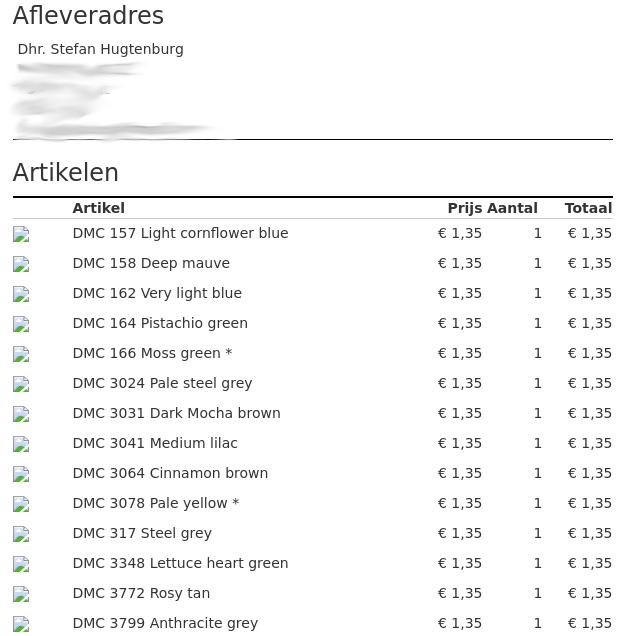
\includegraphics[width=0.8\textwidth]{images/list.png}\\
		\hspace*{15pt}\hbox{\scriptsize Screenshot By:\thinspace{\itshape Stefan Hugtenburg}}
	\end{center}
\end{frame}

\begin{frame}
	\frametitle{Why study the list?}
	\begin{block}{Use cases}
		What do we use lists for?	
	\end{block}
	\pause
	\begin{block}{Many things!}
		\begin{itemize}
			\item To store a collection of data.
				\pause
			\item To build other more complex/refined data structures!
		\end{itemize}
	\end{block}
\end{frame}

\begin{frame}
	\frametitle{Lists in Python}
	\begin{block}{Lists in Python}
		How do lists in Python work?
	\end{block}
	\pause
	\begin{block}{Arrays}
		They are array-based!
	\end{block}
	\pause
	\begin{block}{Arrays?}
		So what's an array then?
	\end{block}
\end{frame}

\begin{frame}
	\frametitle{Arrays}
	\begin{block}{Array}
		An array is a block of memory of fixed size that can hold multiple items of data.
	\end{block}	
	\pause
	\begin{columns}
		\column{0.455\textwidth}
		\vspace{10pt}
		% 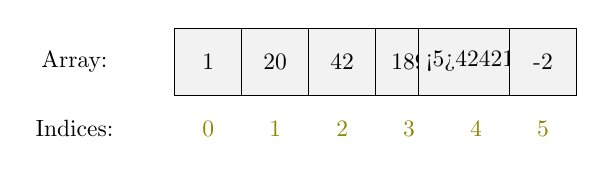
\begin{tikzpicture}[scale=0.85, transform shape]
	\foreach \x/\val in {0/1,1/20,2/42,3/189,4/\alt<5>{\alert{4242}}{17},5/-2}{
	\node[draw,rectangle, fill=gray!10, minimum size =1cm] (c) at (\x,0) {\val};
	\node[olive] (index) at (\x,-1) {\x};
}
\node[] at (-2,0) {Array:};
\node[] at (-2,-1) {Indices:};
\end{tikzpicture}

		\column{0.455\textwidth}
		\pause
		\begin{onlyenv}<3>

			\lstinputlisting{src/array.py}
		\end{onlyenv}
		\begin{onlyenv}<4>

			\lstinputlisting{src/array2.py}
		\end{onlyenv}
		\begin{onlyenv}<5->

			\lstinputlisting{src/array3.py}
		\end{onlyenv}
	\end{columns}
	\only<6>{
		\begin{block}{How is this different?}
			How does this differ from a list?
		\end{block}
	}
	\only<7>{
		\begin{block}{Several ways}
			\begin{itemize}
				\item It's just memory, no things like \texttt{a.sort()}.
				\item It is \textit{finite}!
			\end{itemize}
		\end{block}
	}
\end{frame}

\begin{frame}
	\frametitle{Array-based lists}
	\begin{block}{Array-based list}
		An array-based list (like the \texttt{list} in Python) uses an array internally.
	\end{block}
	\begin{block}{Growing a list?}
		How can we then grow the list (seemingly) infinitely?
		\begin{enumerate}[A.]
			\item The list uses multiple arrays stitched together.
			\item The list also has a finite size from the start, we just never notice.
			\item The list creates a new array of size $n+1$ when the array if full.
			\item The list creates a new array of size $n*2$ when the array if full.
			\item I don't know.
		\end{enumerate}
	\end{block}
\end{frame}

\begin{frame}
	\frametitle{No! Bad Frankenstein!}
	\begin{block}{Stitching arrays together}
		The list uses multiple arrays stitched together.
		\begin{itemize}
			\item Although technically possible, keeping track of all of it is hell not pleasant.
			\item There are also benefits to having one continuous block of memory.
				\begin{itemize}
					\item For instance spacial caching benefits (Google it, if you are intrigued ;))
				\end{itemize}
				\pause
			\item But the idea isn't a bad one per se. Having only single items blocks, forms the basis of the list we study
				after the break!
		\end{itemize}
	\end{block}	
\end{frame}

\begin{frame}
	\frametitle{Too infinity and beyond}
	\begin{block}{A hidden maximum size?}
		The list also has a finite size from the start, we just never notice.
		\begin{itemize}
			\item Nope, we can grow it so long as there is memory available.
		\end{itemize}
	\end{block}	
\end{frame}

\begin{frame}
	\frametitle{So... New arrays then?}
	\begin{block}{A new one!}
		When the initial array is full, we create a new one with more capacity.\\
		We copy over all existing elements into the new array\dots\\
		And we now have new space to grow!
	\end{block}	
	\pause
	\begin{block}{Question}
		But by how much should we grow?	
	\end{block}
	\pause
	\begin{block}{Observations}
		\begin{itemize}
			\item Adding one item, can trigger a full copy of the array...
			\item Does that make \texttt{append} an $O(n)$ operation?
		\end{itemize}
	\end{block}	
\end{frame}

\begin{frame}
	\frametitle{It depends}
	\begin{block}{Just enough room}
		The list creates a new array of size $n+1$ when the array if full.
	\end{block}	
	\begin{block}{Doing it often}
		What happens when we add $n$ elements to a list of size $1$?\\
		\begin{itemize}
			\item Every time we need to copy the full list.
			\item So $O(\sum\limits_{i=1}^{n}i)$ time in total.
			\item So $O(n^2)$ to add $n$ elements\dots
		\end{itemize}
	\end{block}	
\end{frame}

\begin{frame}
	\frametitle{It depends}
	\begin{block}{More than enough room}
		The list creates a new array of size $n*2$ when the array if full.
	\end{block}	
	\begin{block}{Doing it often}
		What happens when we add $n$ elements?
	\end{block}
\end{frame}

\begin{frame}
	\frametitle{Amortised run time}
	\begin{block}{Amortised run time}
		Some operations have varying run times, but can be shown to be efficient when repeated multiple times. We call
		this an amortised run time.
	\end{block}	
	\pause
	\begin{block}{Consider...}
		\small
		\begin{itemize}
			\item Consider a list of size $1$ and we add $n$ elements to it.
				\vspace{-5pt}
				\pause
			\item This means we double the size of the list $\log_2(n)$ times.
				\vspace{-5pt}
				\pause
			\item This means that in total we have: $O(n)$ time to add all elements.
				\vspace{-5pt}
				\pause
			\item And $O\left(\sum\limits_{i=1}^{\log_2(n)} 2^i\right)$ operations to copy when the list grows.
				\vspace{-5pt}
			\item This geometric sequence gets us to: $O(2^{\log_2(n)}) = O(n)$ operations.
				\vspace{-5pt}
				\pause
			\item So $O(n)$ to add $n$ items!
				\vspace{-5pt}
		\end{itemize}
		\pause
		We call this an amortised run time of $O(1)$ for the append operation!
	\end{block}	
\end{frame}

\begin{frame}
	\frametitle{Inserter}
	\begin{center}
		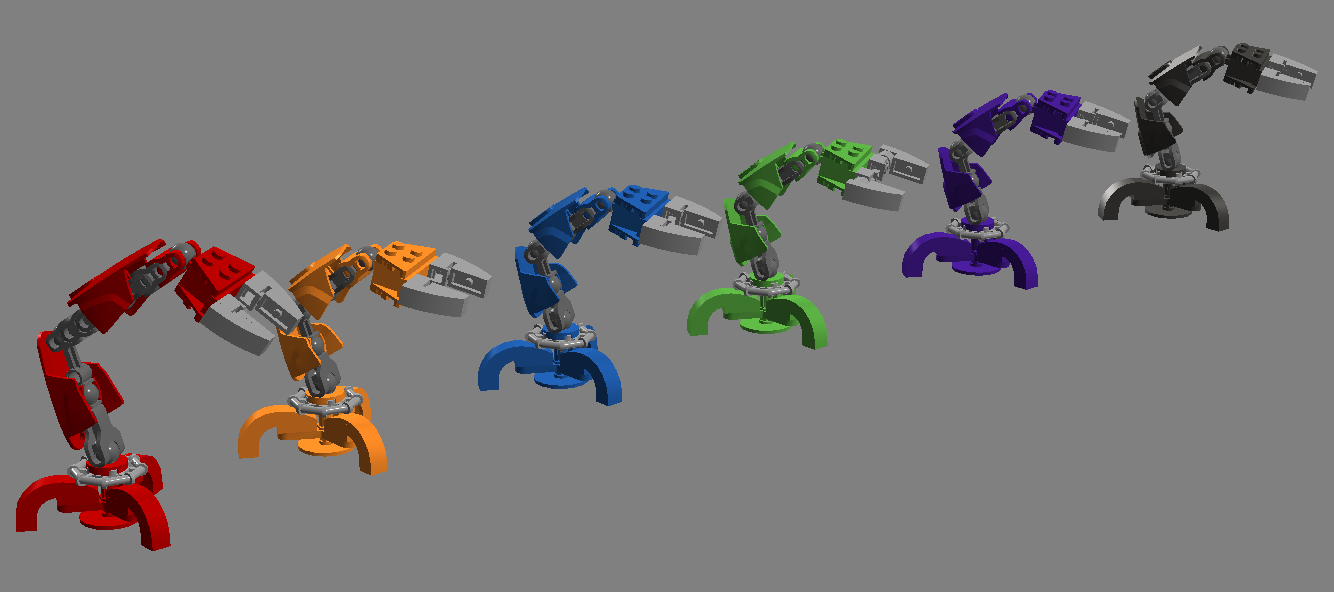
\includegraphics[width=0.8\textwidth]{images/inserter.png}\\
		\hspace*{15pt}\hbox{\scriptsize Image By:\thinspace{\itshape TheMugbearer}}
		% https://www.reddit.com/r/factorio/comments/4s015w/decided_to_also_post_a_sort_of_factorio_fanart/
	\end{center}
\end{frame}

\begin{frame}
	\frametitle{Inserting}
	\begin{columns}
		\column{0.455\textwidth}

		\begin{block}{Let's insert}
			What is the time complexity of \texttt{l.insert(index,value)} when \texttt{len(l)}=n?
			\begin{enumerate}[A.]
				\item $O(1)$
				\item $O(\textit{index})$
				\item $O(n - \textit{index})$
				\item $O(n)$
				\item $O(n^2)$
				\item I don't know.
			\end{enumerate}
		\end{block}
		\pause
		\column{0.455\textwidth}
		\begin{block}{Let's insert}
			We need to shift all elements after \texttt{index}, so $O(n-\textit{index})$
		\end{block}
		\pause
		\begin{block}{Inserting at the front}
			This means prepending is $O(n)$ for array-based lists!
		\end{block}	
	\end{columns}
\end{frame}

\begin{frame}
	\frametitle{Getting rid of the trash}
	\begin{center}
		
\includegraphics[width=0.3\textwidth]{images/trash.jpg}\\
		\hspace*{15pt}\hbox{\scriptsize Image By:\thinspace{\itshape Tgasser}}
		% https://commons.wikimedia.org/wiki/File:Trash_person.jpg
	\end{center}
\end{frame}

\begin{frame}
	\frametitle{Removing an item}
	\begin{columns}
		\column{0.455\textwidth}
		\begin{block}{Let's pop}
			What is the time complexity of \texttt{l.pop(index)} when \texttt{len(l)}=n?
			\begin{enumerate}[A.]
				\item $O(1)$
				\item $O(\textit{index})$
				\item $O(n - \textit{index})$
				\item $O(n)$
				\item $O(n^2)$
				\item I don't know.
			\end{enumerate}
		\end{block}
		\pause
		\column{0.455\textwidth}
		\begin{block}{Let's pop}
			We need to shift all elements after \texttt{index}, so $O(n-\textit{index})$.
		\end{block}
		\pause
		\begin{block}{Inserting at the front}
			This means removing the first item is $O(n)$ for array-based lists!
		\end{block}	
	\end{columns}
\end{frame}

\begin{frame}
	\frametitle{Removing an item}
	\begin{columns}
		\column{0.455\textwidth}
		\begin{block}{Let's remove}
			What is the time complexity of \texttt{l.remove(value)} when \texttt{len(l)}=n?
			\begin{enumerate}[A.]
				\item $O(1)$
				\item $O(\textit{index})$, where index is the index of the value.
				\item $O(n - \textit{index})$, where index is the index of the value.
				\item $O(n)$
				\item $O(n^2)$
				\item I don't know.
			\end{enumerate}
		\end{block}
		\pause
		\column{0.455\textwidth}
		\begin{block}{Let's remove}
			We need to find the element so $O(\textit{index})$.\\
			We need to shift all elements after \texttt{index}, so $O(n-\textit{index})$.\\
			Together this is $O(n)$.
		\end{block}
	\end{columns}
\end{frame}

\begin{frame}
	\frametitle{Freeing up memory}
	\begin{block}{Freeing up space}
		When we remove sufficient items, we can free up space again.\\
		We do this when 25\% of the capacity is used.
	\end{block}	
	\pause
	\begin{block}{Why 25\%?}
		Why not just when we drop below 50\% again?
	\end{block}
	\pause
	\begin{block}{Thrashing}
		Thrashing is repeatedly claiming and releasing memory (and in this case copying the array).\\
		To avoid this, we use a different bound on when we release memory.
	\end{block}
\end{frame}

\begin{frame}
	\frametitle{Lists in Python}
	So to summarise:
	\begin{itemize}
		\item Insert first element: $O(n)$.
		\item Insert at index $k$: $O(n-k)$.
		\item Append: amortised $O(1)$.
		\item Remove first element: $O(n)$.
		\item Remove last element: amortised $O(1)$.
		\item Remove index $k$: $O(n-k)$.
		\item Search (discussed last week): $O(n)$.
	\end{itemize}
\end{frame}

%%%%%%%%%%%%%%%%%%%%%%%%%%%%%%%%%%%%%%%%%%%%%%%%%%%%%%%%%%%%%%%%%%%%%%
\begin{frame}[fragile]\frametitle{}
\begin{center}
{\Large Linked Lists}
\end{center}

\end{frame}

\begin{frame}
	\frametitle{Linked list}
	\begin{center}
		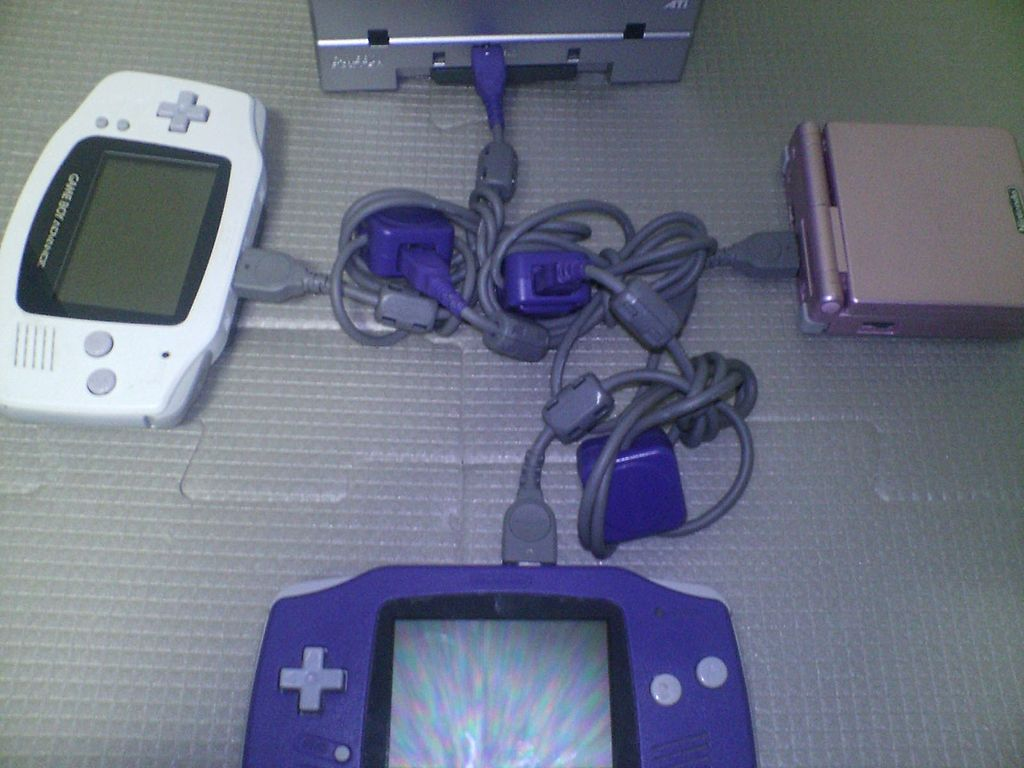
\includegraphics[width=0.6\textwidth]{images/gba.jpg}\\
		\hspace*{15pt}\hbox{\scriptsize Image By:\thinspace{\itshape PiaCarrot}}
		%https://commons.wikimedia.org/wiki/File:GBA_4PConnection.jpg
	\end{center}
\end{frame}

\begin{frame}
	\frametitle{Another approach}
	
	\begin{block}{What do we want to solve?}
		Two things in the array-based implementation that we hope to solve:
		\begin{enumerate}
			\item Only use space for items we actually use.
			\item Allow for efficient ($O(1)$?) adding and removing at the front of the list.
		\end{enumerate}
	\end{block}
	\pause
	\begin{block}{}
		Why do we want this efficient adding/removing?
	\end{block}
\end{frame}

\begin{frame}
	\frametitle{The notion of a linked list}
	\begin{columns}
		\column{0.455\textwidth}
			\begin{itemize}
				\item We build a list of blocks, starting with one item/block (we call this the \alert{head})
				\item<2-> We can then add another.
				\item<3-> These are connected, we can go from the first to the second item.
				\item<4-> So let's add one more item.
				\item<5-> We should also indicate when we have reached the end (we call this the \alert{tail}).
			\end{itemize}
		\column{0.455\textwidth}
		% % Tikz template taken from: https://tex.stackexchange.com/a/19288
\begin{tikzpicture}[list/.style={draw}]

  \node[list] (A) {42};
	\only<2->{
  \node[list] (B) {99};
}
	\only<3->{
  \draw[] let \p1 = (A.two), \p2 = (A.center) in (\x1,\y2) -- (B);
}
	\only<4->{
  \node[list] (C) {12};
  \draw[] let \p1 = (B.two), \p2 = (B.center) in (\x1,\y2) -- (C);
}
\only<5->{
  \node[draw,inner sep=6pt] (D) {};
  \draw (D.north east) -- (D.south west);
  \draw (D.north west) -- (D.south east);
  \draw[] let \p1 = (C.two), \p2 = (C.center) in (\x1,\y2) -- (D);
}
\end{tikzpicture}	

	\end{columns}
\end{frame}

\begin{frame}
	\frametitle{How does this work now?}
	\framesubtitle{Searching for an item}	
	The approach:
	\begin{enumerate}
		\item Start at the head of the list.
		\item<2-> If this is is the item we need, return True.
		\item<2-> Else if this is the tail, return False.
		\item<3-> Else, move to the next item of the list and go to step 2.
	\end{enumerate}

		% % Tikz template taken from: https://tex.stackexchange.com/a/19288
\begin{tikzpicture}[list/.style={draw}]

	\node[list,on chain,onslide=<1-2>{red}] (A) {42};
	\node[list,on chain,onslide=<3>{red}] (B) {99};
  \draw[] let \p1 = (A.two), \p2 = (A.center) in (\x1,\y2) -- (B);
  \node[list,on chain,onslide=<4>{red}] (C) {12};
  \draw[] let \p1 = (B.two), \p2 = (B.center) in (\x1,\y2) -- (C);
	\node[on chain,draw,inner sep=6pt,onslide=<5>{red}] (D) {};
	\draw[onslide=<5>{red}] (D.north east) -- (D.south west);
	\draw[onslide=<5>{red}] (D.north west) -- (D.south east);
  \draw[] let \p1 = (C.two), \p2 = (C.center) in (\x1,\y2) -- (D);
\end{tikzpicture}	

	
	\only<6->{
	\lstinputlisting{src/ll_search.py}
}
\end{frame}

\begin{frame}
	\frametitle{Getting an item!?}
	\framesubtitle{Getting item at index $i$}

	\begin{itemize}
		\item There is no easy way to access the $i$th item other than to `walk' there.
		\item So $O(\textit{index})$ to get the item at a certain \texttt{index}.
	\end{itemize}
	\lstinputlisting{src/ll_get.py}
\end{frame}

\begin{frame}
	\frametitle{Inserting at the head or tail}
	\begin{itemize}
		\item Take the current head or tail.
		\item And put the new node before or after it :)
		\item<4-> \alert{$O(1)$ time!}
	\end{itemize}	
	\begin{columns}[t]
		\column{0.535\textwidth}
	\only<2->{
		\lstinputlisting{src/ll_prepend.py}
	}
		\column{0.535\textwidth}
	\only<3->{
		\lstinputlisting{src/ll_append.py}
	}
			
	\end{columns}
\end{frame}

\begin{frame}
	\frametitle{Assumptions, Assumptions}
	\begin{block}{Unfortunately}
		To do \texttt{add\_last} in constant time, we need a reference to the \texttt{tail}.\\
		Many implementations of Singly-Linked Lists do not have this.
	\end{block}		
	\pause
	\begin{block}{Wait Singly?}
		What do I mean with `Singly' Linked List?	
	\end{block}
	\pause
	\begin{block}{Well, it's not doubly linked}
		In other implementations, we can both go forwards and backwards!	
	\end{block}
\end{frame}

\begin{frame}
	\frametitle{Doubly-Linked Lists}
	\begin{overlayarea}{\textwidth}{0.5\textheight}
		% \begin{center}
			% % Tikz template taken from: https://tex.stackexchange.com/a/19288
\begin{tikzpicture}[list/.style={rectangle split, rectangle split parts=2,
    draw, rectangle split horizontal}, >=stealth, start chain]

  \node[list,on chain] (A) {42};
  \node[list,on chain] (B) {99};
  \draw[*->] let \p1 = (A.two), \p2 = (A.center) in (\x1,\y2) -- (B);
  \node[list,on chain] (C) {12};
  \draw[*->] let \p1 = (B.two), \p2 = (B.center) in (\x1,\y2) -- (C);
  \node[on chain,draw,inner sep=6pt] (D) {};
  \draw (D.north east) -- (D.south west);
  \draw (D.north west) -- (D.south east);
  \draw[*->] let \p1 = (C.two), \p2 = (C.center) in (\x1,\y2) -- (D);

\end{tikzpicture}	

		% \end{center}
		\only<1->{
			\begin{block}{A singly linked list}
				Only has connections in one direction.	
			\end{block}	
		}
		\only<2>{
			% \begin{center}
				% % Tikz template taken from: https://tex.stackexchange.com/a/19288
\begin{tikzpicture}[list/.style={rectangle split, rectangle split parts=2,
    draw, rectangle split horizontal},start chain]

		\only<2->{
  \node[on chain,draw,inner sep=6pt] (E) {};
  \draw (E.north east) -- (E.south west);
  \draw (E.north west) -- (E.south east);
}
  \node[list,on chain] (A) {42};
  \node[list,on chain] (B) {99};
  \draw[*->] let \p1 = (A.two), \p2 = (A.center) in (\x1,\y2) -- (B);
  \node[list,on chain] (C) {12};
  \draw[*->] let \p1 = (B.two), \p2 = (B.center) in (\x1,\y2) -- (C);
  \node[on chain,draw,inner sep=6pt] (D) {};
  \draw (D.north east) -- (D.south west);
  \draw (D.north west) -- (D.south east);
  \draw[*->] let \p1 = (C.two), \p2 = (C.center) in (\x1,\y2) -- (D);

	\only<2->{
		\draw[->,red,thick] let \p1 = (A.two), \p2 = (A.center) in (B) to [out=150, in=30] (\x1,\y2);
		\draw[->,red,thick] let \p1 = (B.two), \p2 = (B.center) in (C) to [out=150, in=30] (\x1,\y2);
		\draw[->,red,thick] let \p1 = (E.center), \p2 = (E.center) in (A) to [out=150, in=30] (\x1,\y2);
	}
\end{tikzpicture}	

			% \end{center}
			\begin{block}{A doubly linked list}
				Has connections in both directions.
			\end{block}
		}
	\end{overlayarea}
\end{frame}

\begin{frame}
	\frametitle{Inserting an item}
	\framesubtitle{What to do?}
	\begin{columns}
		\column{0.255\textwidth}
	\begin{itemize}
		\item Navigate to the place where we want to insert the item ($O(\textit{index})$)
			\pause
		\item Add the item: $O(1)$
			\pause
		\item So $O(\textit{index})$ time!
	\end{itemize}
			
		\column{0.755\textwidth}
		\pause
	\lstinputlisting{src/ll_insert.py}
			
	\end{columns}
\end{frame}

\begin{frame}
	\frametitle{Removing an item}
	\begin{block}{Removing an item}
		What is the time complexity of removing the first and last item in a singly linked list?
		\only<1>{
		\begin{enumerate}[A.]
			\item $O(1)$ for the first, $O(1)$ for the last.
			\item $O(1)$ for the first, $O(n)$ for the last.
			\item $O(n)$ for the first, $O(1)$ for the last.
			\item $O(n)$ for the first, $O(n)$ for the last.
			\item I don't know.
		\end{enumerate}
	}
	\end{block}
	\vspace{-20pt}
	\begin{columns}[t]
		
		\column{0.535\textwidth}
	\only<2->{
		\lstinputlisting{src/ll_remove_first.py}
	\vspace{-5pt}
		$O(1)$ time.
	}
		\column{0.535\textwidth}
	\only<3->{
		\lstinputlisting{src/ll_remove_last.py}
	\vspace{-5pt}
		$O(n)$ time.
	}
	\end{columns}
	
\end{frame}

\begin{frame}
	\frametitle{Improvements!}
		\begin{block}{Doubly-linked list remove last}
			Note that in a doubly-linked list we can remove the last item in $O(1)$ time!\\
			We can just use \texttt{tail.prev} to find the last-but-one element in constant time!\\
		\end{block}	
\end{frame}

\begin{frame}
	\frametitle{So to summarise}
\begin{columns}
	\column{0.655\textwidth}
	\begin{tabular}{l | c | c | c}
	Operation & Array-based list & SLL & DLL \\	
	\midrule
	Get element $k$ & $O(1)$ &$O(k)$ & $O(k)$ \\
	\pause
	Insert first element& $O(n)$ & $O(1)$ & $O(1)$\\
	Insert at index $k$& $O(n-k)$ & $O(k)$ & $O(\min(k,n-k))$\\
	Append (amortised)& $O(1)$ & $O(1)$ & $O(1)$\\
	\pause
	Remove first element& $O(n)$ & $O(1)$ & $O(1)$\\
	Remove last element& $O(1)$ & $O(n)$ & $O(1)$\\
	Remove index $k$& $O(n-k)$ & $O(k)$ & $O(\min(k,n-k))$\\
	\pause
	Search & $O(n)$ & $O(n)$ & $O(n)$\\
	\end{tabular}
		
	\column{0.355\textwidth}
%	\pause
%	\begin{block}{Which should you use?}
%		So which is better?	
%	\end{block}
%	\pause
%	\begin{block}{It depends!}
%		But on what?	
%	\end{block}
		
\end{columns}

\end{frame}

%%%%%%%%%%%%%%%%%%%%%%%%%%%%%%%%%%%%%%%%%%%%%%%%%%%%%%%%%%%%%%%%%%%%%%
\begin{frame}[fragile]\frametitle{}
\begin{center}
{\Large Queue}
\end{center}

\end{frame}

\begin{frame}
	\frametitle{The Queue ADT}
	\begin{overlayarea}{\textwidth}{\textheight}
		\begin{block}{The Queue}
			\begin{itemize}
				\item \texttt{size()} (or \texttt{len(s)}) to get the number of items in the queue.
				\item \texttt{enqueue(item)} to add something to the queue.
					\pause
				\item \texttt{dequeue()} to remove the first element from the queue.
				\item \texttt{peek()} to view the first element of the queue.
			\end{itemize}
		\end{block}	
		\pause
		\begin{block}{Data structure?}
			What kind of data structure should we use to implement a Queue?
				\only<3>{
				\begin{enumerate}[A.]
					\item An array
					\item A python list
					\item A linked list
					\item A dict
				\end{enumerate}
			}
		\end{block}
		\pause
		\begin{block}{One end only}
			Only removing on one end and adding on the other? Seems like a DLL will do.
		\end{block}
	\end{overlayarea}
\end{frame}

\begin{frame}
	\frametitle{Implementing a Linked-List based Queue}
	\begin{overlayarea}{\textwidth}{\textheight}
			\begin{tabular}{r | c c}
				Queue operation & DLL operation & Time Complexity \\
				\midrule
				\texttt{size} & \only<2->{\texttt{size} & $O(1)$} \\
				\texttt{enqueue} & \only<2->{\texttt{add\_last} & $O(1)$} \\
				\texttt{dequeue}  & \only<2->{\texttt{remove\_first} & $O(1)$} \\
				\texttt{peek}  & \only<2->{\texttt{head} & $O(1)$} \\
			\end{tabular}
		
			\begin{columns}[t]
				\column{0.455\textwidth}
			\only<3->{
			\begin{block}{Arrays}
				Could we also do this using an array-based list?	
			\end{block}
		}
			\only<5->{
			\begin{block}{SLL}
				What about an SLL?
			\end{block}
		}
				\column{0.455\textwidth}
				\only<4->{
				\begin{block}{No more growing}
					Sure, but only for fixed capacity queues.
				\end{block}
				}
				\only<6->{
				\begin{block}{Eeyore}
					Only if we have the tail pointer.
				\end{block}
				}
		
			\end{columns}
	\end{overlayarea}
\end{frame}

\begin{frame}
	\frametitle{Snake games}
	\framesubtitle{Nostalgia overload}
	\begin{center}
		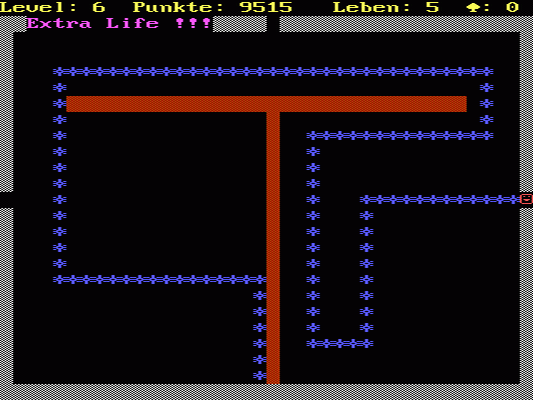
\includegraphics[width=0.6\textwidth]{images/snake.png}\\
		\hspace*{15pt}\hbox{\scriptsize Image By:\thinspace{\itshape Thomas Jensen}}
	\end{center}
	% https://commons.wikimedia.org/wiki/File:Cgasnake.png 
\end{frame}

\begin{frame}
	\frametitle{Why a queue}
		\begin{block}{In snake...}
			\begin{itemize}
				\item In snake, the body of the snake follows the head.
					\pause
				\item If we first go left, then right, then every part of the body also needs to go first left then right.
					\pause
				\item This is like a queue!
			\end{itemize}
		\end{block}	
		\pause
			\begin{block}{Many others?}
				But of course there are many other real-world examples.
				\begin{itemize}
					\item Ticket counters,
					\item Traffic jams,
					\item Coffee machines and printers,
					\item Take-out restaurants,
					\item etc.
				\end{itemize}
			\end{block}	
\end{frame}

\begin{frame}
	\frametitle{Double-Ended Queues}

	\begin{center}
		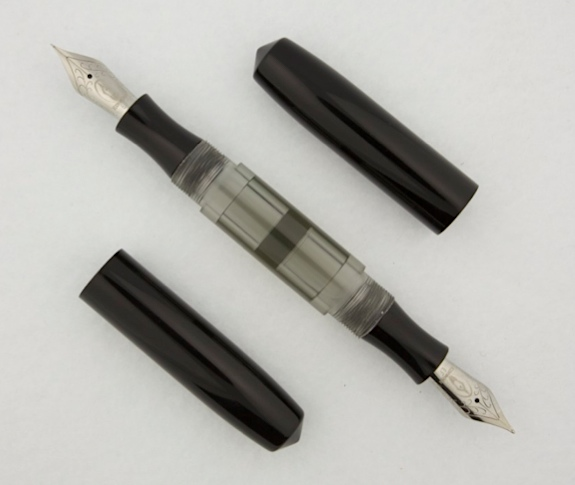
\includegraphics[width=0.5\textwidth]{images/de.jpg}\\
		\hspace*{15pt}\hbox{\scriptsize Image By:\thinspace{\itshape Chris Lott}}
		% https://www.flickr.com/photos/fncll/9824392125
	\end{center}
\end{frame}

\begin{frame}
	\frametitle{Deques}
		\begin{block}{Deques}
			Deques, or Double-Ended Queues, allow both FIFO and LIFO operations in $O(1)$ time.
		\end{block}		
		\pause
		\begin{block}{Hang on...}
			Doesn't that sound familiar?	
		\end{block}
		\pause
		\begin{block}{Back to DLL}
			This is exactly what a DLL offers!
		\end{block}
\end{frame}

\begin{frame}
	\frametitle{\texttt{deque}}
	
	In python we can use a \texttt{deque} called \texttt{d} on which:
	\begin{itemize}
		\item We can \textit{push} with \texttt{d.append}.
		\item We can \textit{pop} with \texttt{d.pop}.
		\item We can \textit{top} with \texttt{d[-1]}
			\pause
		\item We can \textit{enqueue} with \texttt{d.append}.
		\item We can \textit{dequeue} with \texttt{d.popleft}.
		\item We can \textit{peek} with \texttt{d[0]}
			\pause
		\item Oh yeah and if you want, you can also add to the left with \texttt{appendleft}
	\end{itemize}
\end{frame}


%%%%%%%%%%%%%%%%%%%%%%%%%%%%%%%%%%%%%%%%%%%%%%%%%%%%%%%%%%%%%%%%%%%%%%
\begin{frame}[fragile]\frametitle{}
\begin{center}
{\Large Stack}
\end{center}

\end{frame}


\begin{frame}
	\frametitle{Stacks}
	\begin{center}
		
\includegraphics[width=0.4\textwidth]{images/stack_of_books.png}\\
		\hspace*{15pt}\hbox{\scriptsize Image from \thinspace{\itshape Pixabay}}
		% https://pixabay.com/en/books-stacked-pile-stacks-25159/
	\end{center}
\end{frame}

\begin{frame}
	\frametitle{Me and my books}
	\framesubtitle{A life-long story}

	\begin{columns}
		\column{0.455\textwidth}
			\begin{center}
				\alt<4->{
					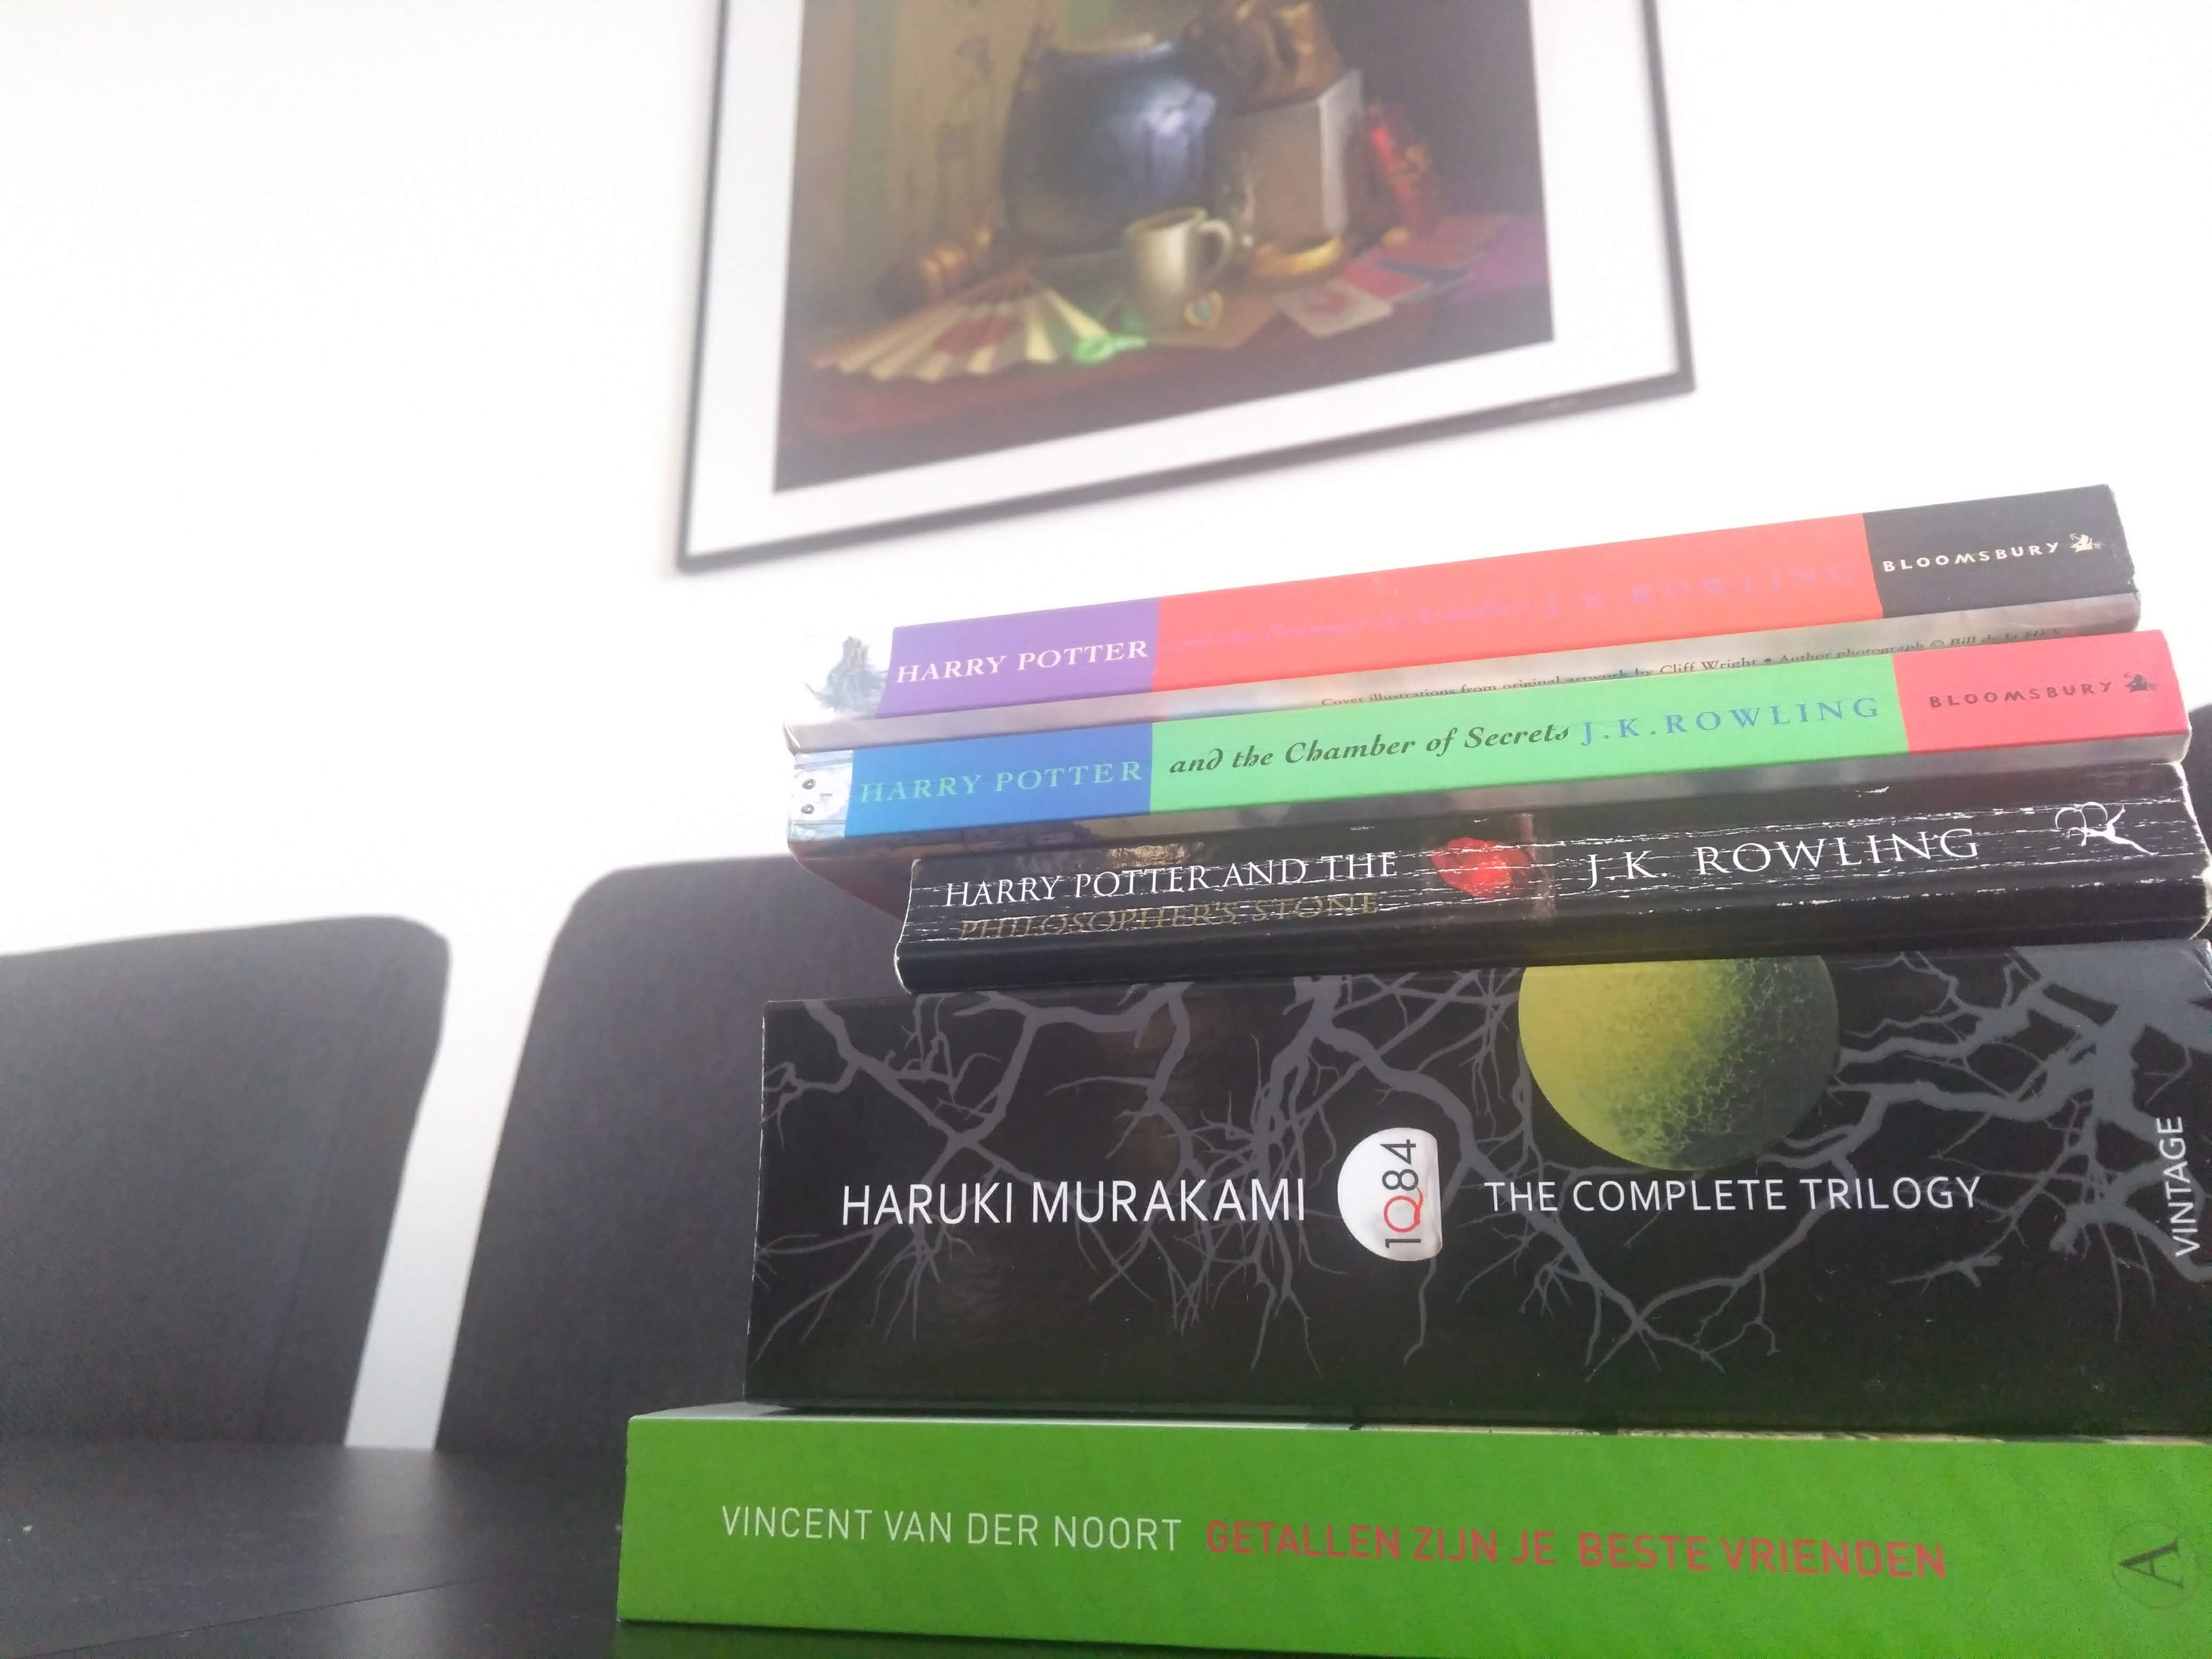
\includegraphics[width=\textwidth]{images/stack_read.jpg}\\
					}{
					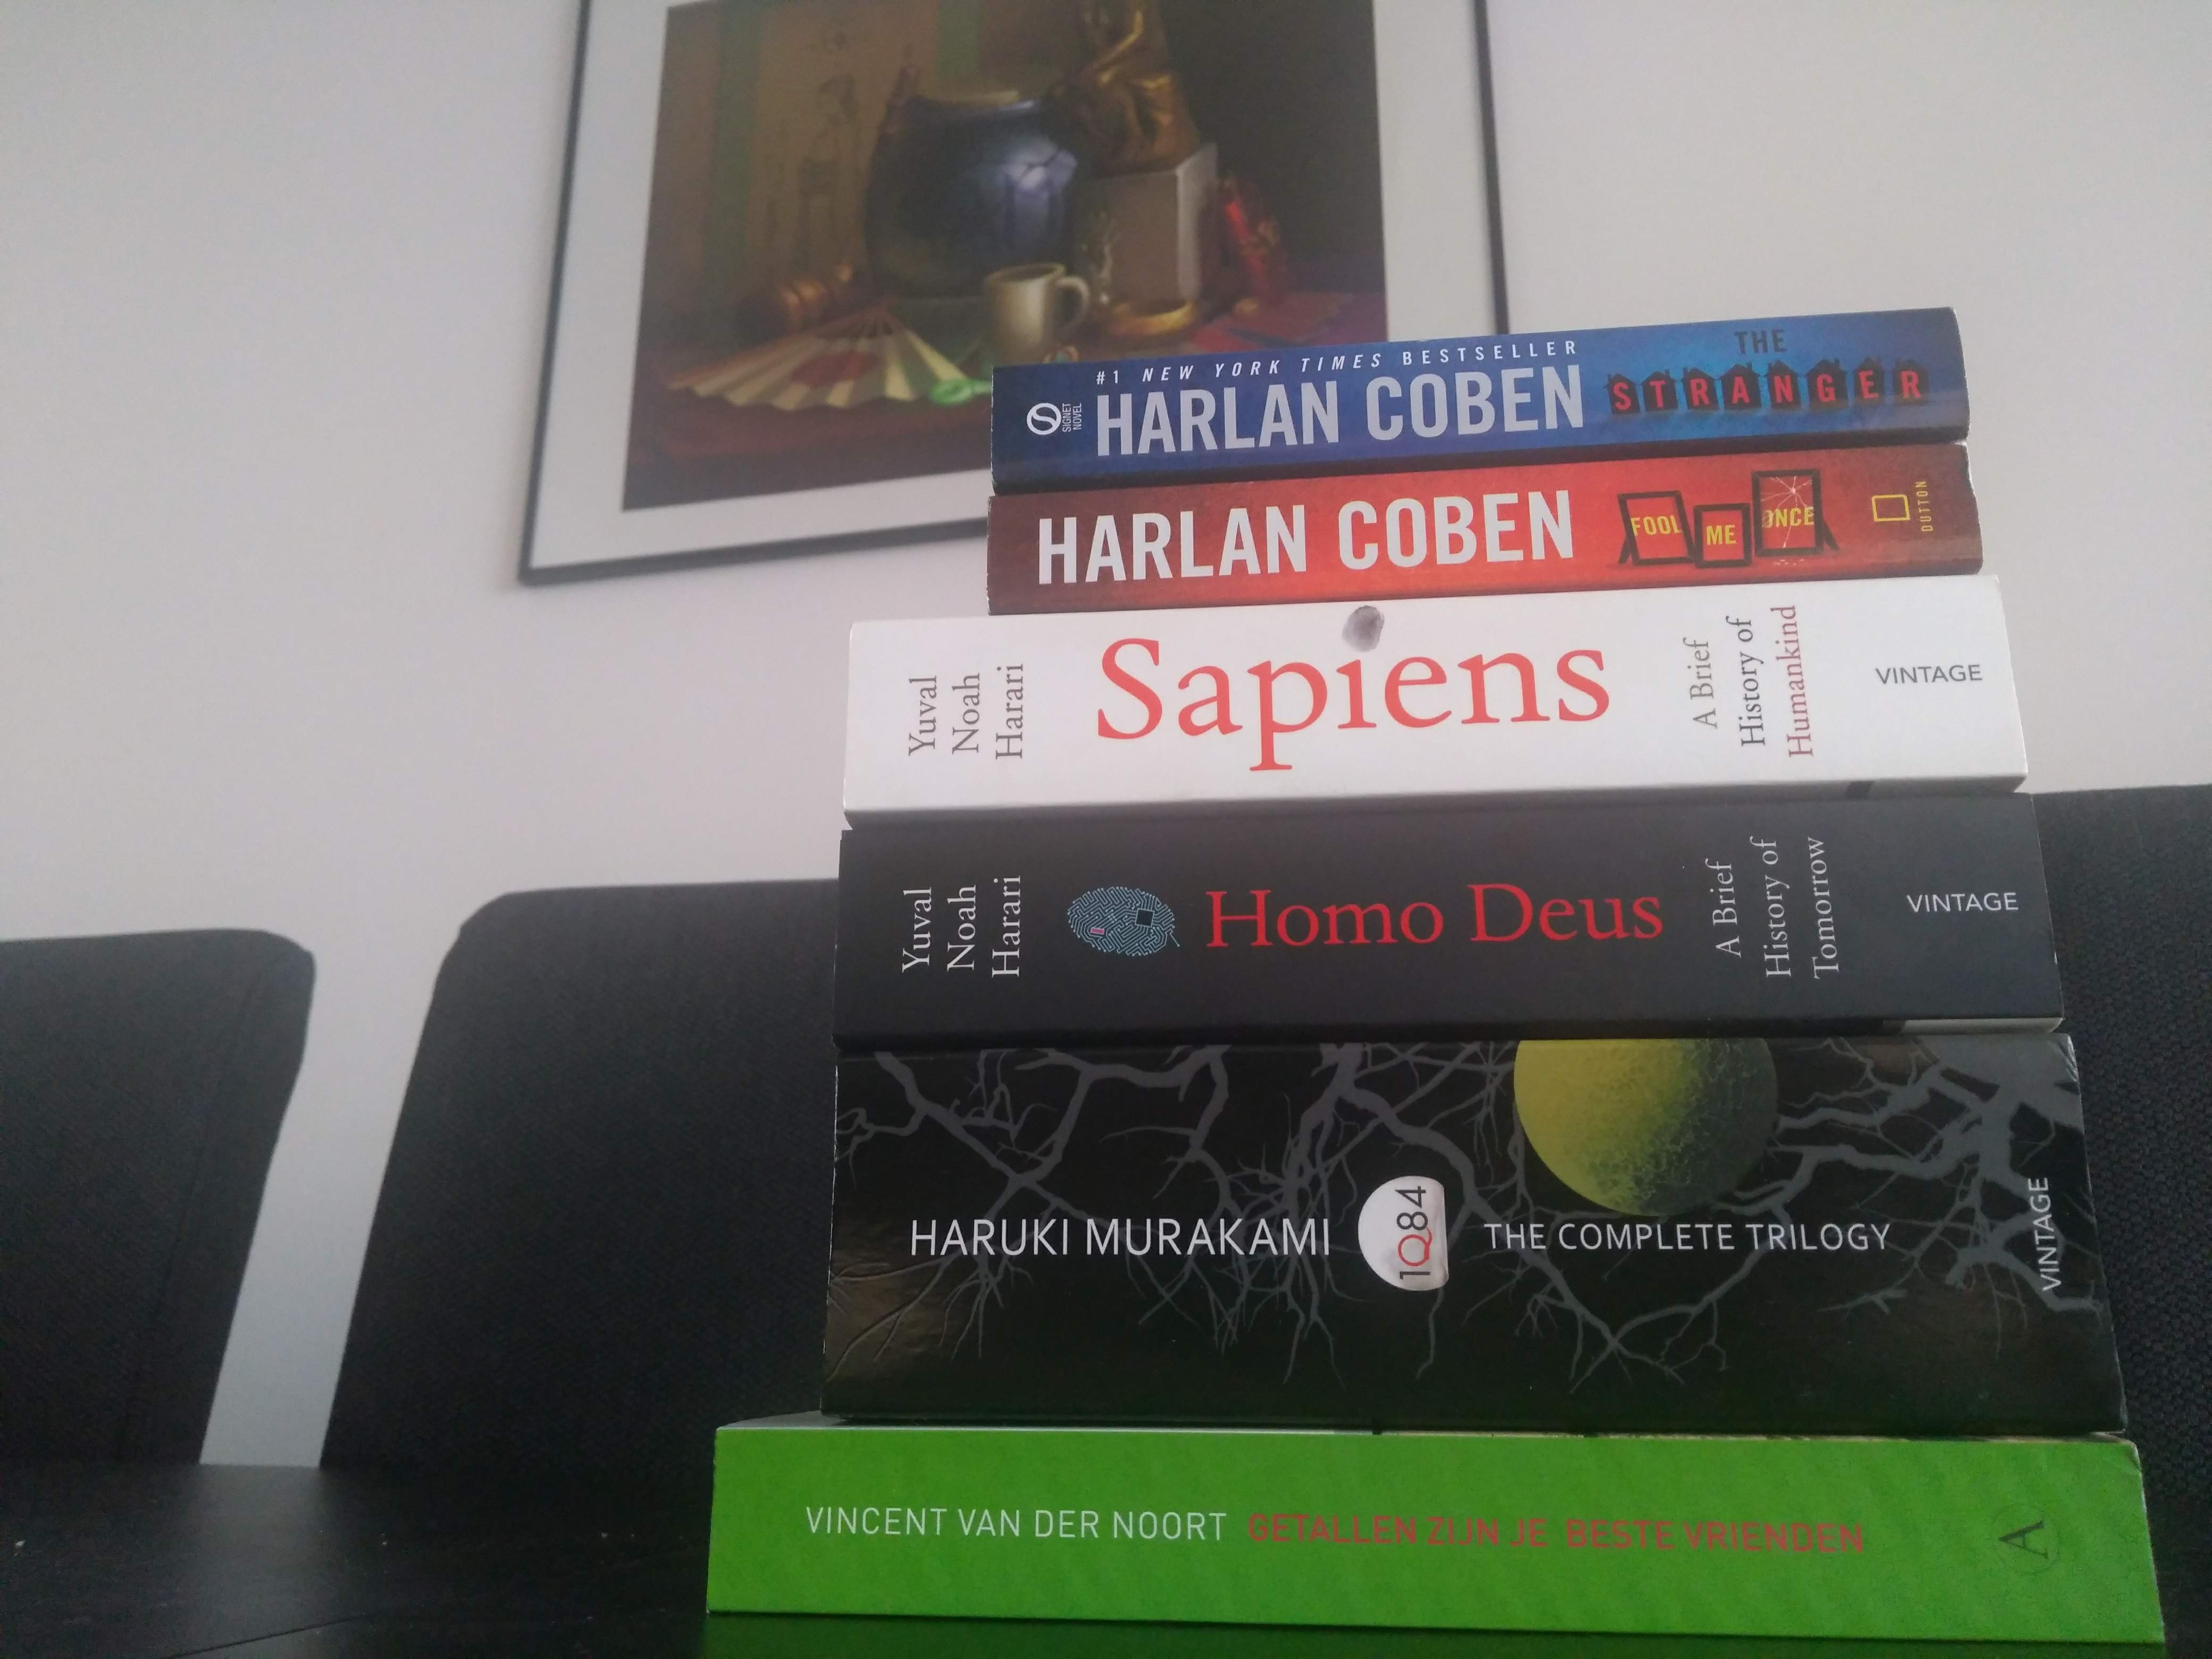
\includegraphics[width=\textwidth]{images/stack_unread.jpg}\\
					}
				\hspace*{15pt}\hbox{\scriptsize Image By:\thinspace{\itshape Stefan Hugtenburg}}
				\hspace*{15pt}\hbox{\scriptsize Bookcovers and picture in the back by others}
			\end{center}
		\column{0.455\textwidth}
		\begin{itemize}
			\item This is how I used to store books I still wanted to read.
				\pause
			\item A nice \alert{stack} of books, with new ones going on the top.
				\pause
			\item After finishing one, I would take the next one from the top.
				\pause
			\item So after a few weeks\dots
				\pause
			\item This uses the \alert{LIFO}-principle.
		\end{itemize}
	\end{columns}
\end{frame}

\begin{frame}
	\frametitle{The what!?}
	\framesubtitle{LIFO}
	
		\begin{block}{LIFO}
			The \textit{Last-In-First-Out}, or LIFO, principle is the working of a stack.\\
			\pause
			The last thing we've added to the stack is the first thing we take out.\\
			\pause
			Similarly the first we have added to the stack, is the last to be taken out.
		\end{block}	
\end{frame}

\begin{frame}
	\frametitle{The Stack ADT}
	\begin{overlayarea}{\textwidth}{\textheight}
		\only<1>{
			\begin{block}{ADT}
				An ADT, or Abstract Data Type, is a description of the behaviour of a data structure.
			\end{block}	
		}
		\pause
			\begin{block}{The Stack}
				\begin{itemize}
					\item \texttt{size()} (or \texttt{len(s)}) to get the number of items in the stack.
					\item \texttt{push(item)} to add something to the stack.
						\pause
					\item \texttt{pop()} to remove the top element from the stack.
					\item \texttt{top()} to view the top element of the stack.
				\end{itemize}
			\end{block}	
			\pause
			\begin{block}{Data structure?}
				What kind of data structure should we use to implement a Stack?
				\only<4>{
				\begin{enumerate}[A.]
					\item An array
					\item A python list
					\item A linked list
					\item A dict
				\end{enumerate}
			}
			\end{block}
			\pause
			\begin{block}{One end only}
				Only removing and adding on one end? Seems like a DLL will do.
			\end{block}
	\end{overlayarea}
\end{frame}

\begin{frame}
	\frametitle{Implementing a Linked-List based Stack}
	\begin{overlayarea}{\textwidth}{\textheight}
			\begin{tabular}{r | c c}
				Stack operation & DLL operation & Time Complexity \\
				\midrule
				\texttt{size} & \only<2->{\texttt{size} & $O(1)$} \\
				\texttt{push} & \only<2->{\texttt{add\_last} & $O(1)$} \\
				\texttt{pop}  & \only<2->{\texttt{remove\_last} & $O(1)$} \\
				\texttt{top}  & \only<2->{\texttt{tail} & $O(1)$} \\
			\end{tabular}
		
			\begin{columns}[t]
				\column{0.455\textwidth}
			\only<3->{
			\begin{block}{Arrays}
				Could we also do this using an array-based list?	
			\end{block}
		}
			\only<5->{
			\begin{block}{SLL}
				What about an SLL?
			\end{block}
		}
				\column{0.455\textwidth}
				\only<4->{
				\begin{block}{Amortised}
					Sure, but it's only amortised $O(1)$. So why would we?
				\end{block}
				}
				\only<6->{
				\begin{block}{Front = Back}
					Sure, but we add and remove from the front!
				\end{block}
				}
		
			\end{columns}
	\end{overlayarea}
\end{frame}

%%%%%%%%%%%%%%%%%%%%%%%%%%%%%%%%%%%%%%%%%%%%%%%%%%%%%%%%%%%%%%%%%%%%%%
\begin{frame}[fragile]\frametitle{}
\begin{center}
{\Large Maps}
\end{center}

\end{frame}


\begin{frame}
	\frametitle{Maps}
	
	\begin{center}
		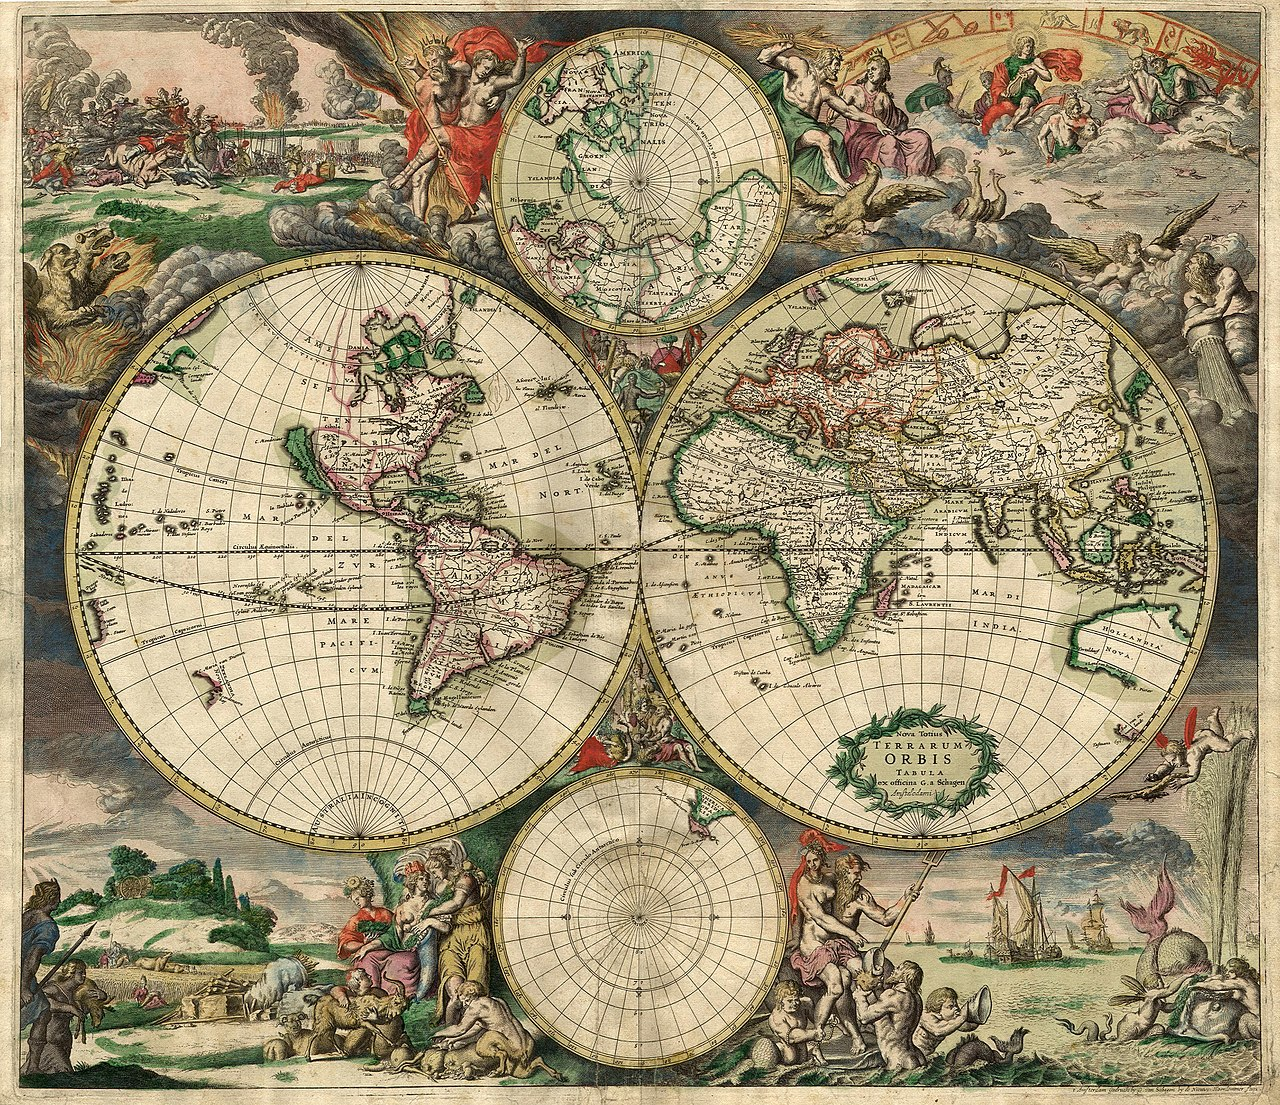
\includegraphics[width=0.5\textwidth]{images/world_map.JPG}\\
		\hspace*{15pt}\hbox{\scriptsize Image By:\thinspace{\itshape Gerard van Schagen}}
		%https://commons.wikimedia.org/wiki/File:World_Map_1689.JPG
	\end{center}
\end{frame}

\begin{frame}
	\frametitle{The map ADT}
	
		\begin{block}{The map ADT}
			Maps work on \textit{key-value} pairs, usually denoted as tuples: $(k,v)$.
			\pause
			\begin{itemize}
				\item \texttt{M.size()} (or \texttt{len(M)}) to get the number of tuples in the map.
					\pause
				\item \texttt{M.get(k)} (or \texttt{M[k]}) to retrieve the value for key $k$.
				\item \texttt{M.put(k,v)} (or \texttt{M[k] = v}) to set the value for key $k$ to $v$.
					\pause
				\item \texttt{M.remove(k)} (or \texttt{del M[k]}) to remove the tuple with key $k$.
					\pause
				\item \texttt{M.contains(k)} (or \texttt{k in M}) to determine if there is tuple with key $k$.
			\end{itemize}
		\end{block}	
\end{frame}

\begin{frame}
	\frametitle{A naive implementation}
	\framesubtitle{Listing a map}

	\begin{block}{Why not just use a list?}
		If we use a list to implement the map where we just throw in all the tuples, what would the time complexity
		of the functions \texttt{get}, \texttt{remove}, \texttt{contains} be?
		\pause
		\begin{enumerate}[A.]
			\item $\Theta(1)$
			\item $\Theta(\log n)$
			\item $\Theta(n)$
			\item $\Theta(n^2)$
			\item I don't know
		\end{enumerate}
	\end{block}
	\pause
	\begin{block}{Not so great}
		All would take linear time! \\
		We would just have to check all the objects every time!
	\end{block}
\end{frame}

\begin{frame}
	\frametitle{Can we do better?}
	\begin{block}{Can we do better?} 
		Can we do better, and if so how?
	\end{block}	
	\pause
	\begin{block}{Yes!}
		How about we try to use an array-based structure where the key determines the index?\\
		\pause
		This allows for $\Theta(1)$ operations for getting, removing or checking an item!
	\end{block}
	\pause
	\begin{block}{But...}
		But what if the key is not integer?
	\end{block}
\end{frame}


\begin{frame}
	\frametitle{A hash}
\begin{center}
	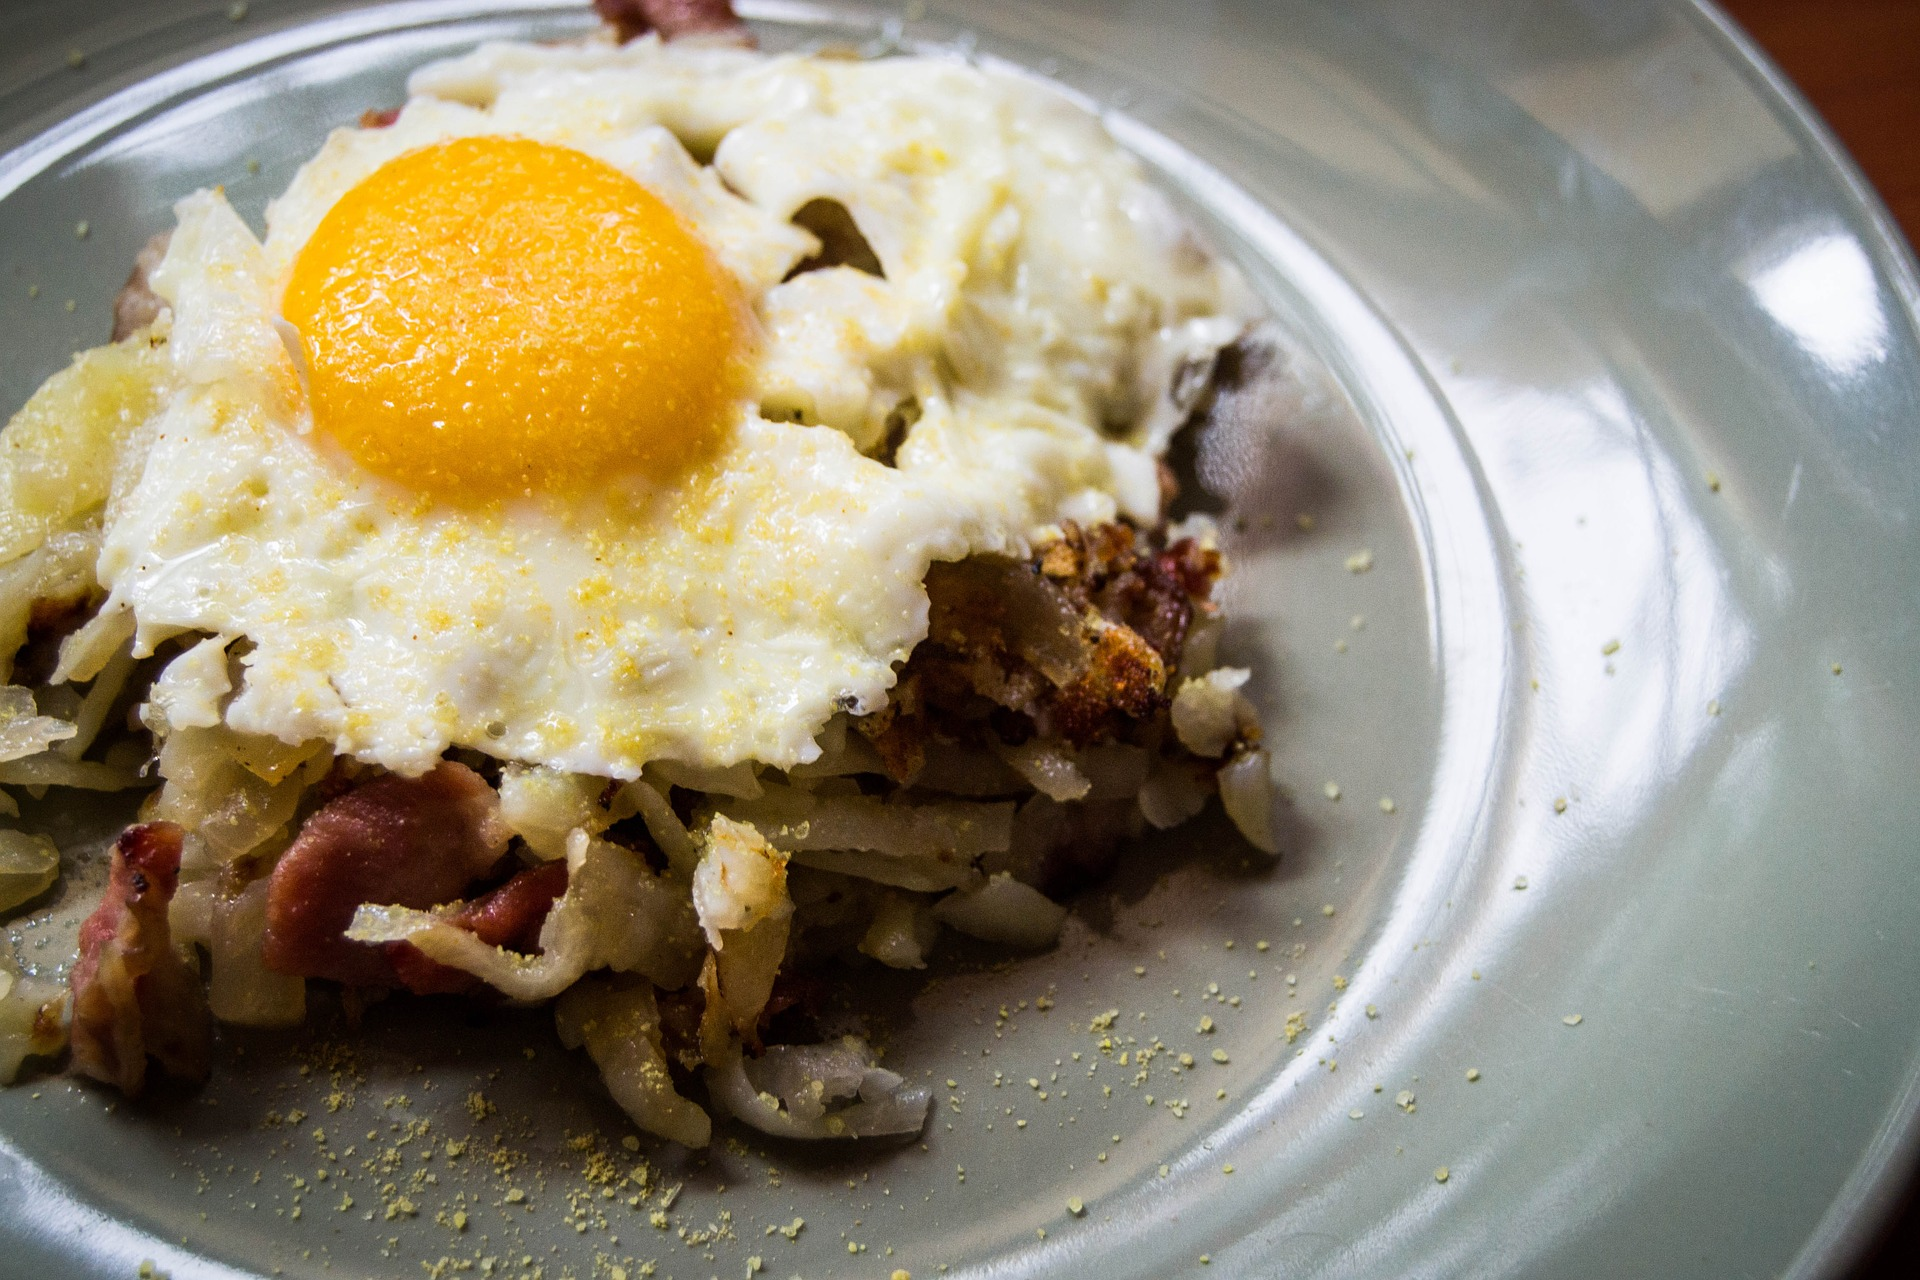
\includegraphics[width=0.6\textwidth]{images/hash.jpg}\\
	\hspace*{15pt}\hbox{\scriptsize Image By:\thinspace{\itshape ailinder}}
	% https://pixabay.com/photos/hash-eggs-food-meal-potato-plate-1330575/
\end{center}
\end{frame}

\begin{frame}
	\frametitle{Hash functions}
	
		\begin{block}{Hash functions}
			Hash functions map each key $k$ to a an integer in a range $[0, N-1]$ for some $N$.\\
		\end{block}	
		\pause
		\begin{block}{That's easy right?}
			Consider the hash function $f(k) = 1$ for any key $k$.\\
			Is this a hash function for $N=100$?
			\begin{enumerate}[A.]
				\item Yes
				\item No
				\item I don't know
			\end{enumerate}
		\end{block}

		\pause
			\begin{block}{It is...}
				It is a hash function, but a terrible one!\\
				Why?
			\end{block}	
\end{frame}

\begin{frame}
	\frametitle{Hash to determine the index}

	\begin{block}{A hash table}
		We want to use hash functions to map keys to a certain index in a hash table.
	\end{block}
	\pause
	\begin{block}{Back to hundred-acre woods}
		Take $f(p) = 1$, $f(i) = 3$, $f(g) = 2$, $f(l) = 8$, $f(e) = 5$, $f(t) = 7$.
		\pause
		This would create the hash table:
		\begin{center}
			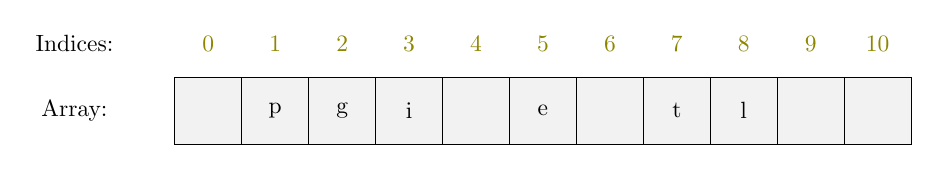
\begin{tikzpicture}[scale=0.85, transform shape]
	\foreach \x/\val in {0/,1/p,2/g,3/i,4/,5/e,6/,7/t,8/l,9/,10/}{
	\node[olive] (index) at (\x,1) {\x};
	\node[draw,rectangle, fill=gray!10, minimum size =1cm] (c) at (\x,0) {\val};
}
\node[] at (-2,1) {Indices:};
\node[] at (-2,0) {Array:};
\end{tikzpicture}

		\end{center}
	\end{block}	
	\pause
	\begin{block}{The simple mapping}
		But what if we have conflicts? Like by taking $f(k)=1$ for all $k$.
	\end{block}	
\end{frame}

\begin{frame}
	\frametitle{Hashing conflicts}
	\begin{block}{A hash table}
		We want to use hash functions to map keys to a certain index in a hash table.\\
		But what do we do if we have hashing conflicts?
	\end{block}
	\pause
	\begin{block}{Back to hundred-acre woods}
		Take $f(e) = 1$, $f(y) = 3$, $f(o) = \alert{3}$, $f(r) = 8$.
		\pause
		This would create the hash table:
		% \begin{center}
			% \begin{tikzpicture}[scale=0.85, transform shape]
	\foreach \x/\val in {0/,1/,2/,3/,4/,5/,6/,7/,8/,9/,10/}{
	\node[olive] (index) at (\x,1) {\x};
	\node[draw,rectangle, fill=gray!10, minimum size =1cm] (\x) at (\x,0) {\val};
}
\node[] at (-2,1) {Indices:};
\node[] at (-2,0) {Array:};

\node[draw,rectangle, fill=gray!10, minimum size =0.5cm] at (1,-1.5) (e) {e};
\node[draw,rectangle, fill=gray!10, minimum size =0.5cm] at (3,-1.5) (A) {y};
\node[draw,rectangle, fill=gray!10, minimum size =0.5cm] at (3,-2.5) (B){o};
\node[draw,rectangle, fill=gray!10, minimum size =0.5cm] at (8,-1.5) (r) {r};
\draw[->, ultra thick] (A) -- (B);
\draw[*->, ultra thick] (1.center) -- (e);
\draw[*->, ultra thick] (3.center) -- (A);
\draw[*->, ultra thick] (8.center) -- (r);
\end{tikzpicture}

		% \end{center}
	\end{block}	
\end{frame}

\begin{frame}
	\frametitle{Hash tables}
	\begin{block}{Hash tables}
		We have an array of a certain capacity.\\
		The hash of a key, determines which \textit{bucket} to use.\\
		\pause
		Every entry could for instance hold a linked-list of values.
	\end{block}		
	\pause
	\begin{columns}
		\column{0.455\textwidth}
			
	\begin{block}{What happens?}
		So for $f(k) = 1$ for all $k$, what is the time complexity of getting the right value out for our key?
		\begin{enumerate}[A.]
			\item $\Theta(1)$
			\item $\Theta(\log n)$
			\item $\Theta(n)$
			\item $\Theta(n^2)$
		\end{enumerate}
	\end{block}
		\column{0.455\textwidth}
			
		\pause
		\begin{block}{Still linear}
			It is still linear time! All end up in a list after all.
		\end{block}
	\end{columns}
\end{frame}

\begin{frame}
	\frametitle{Hash functions: Ideal properties}
	
		\begin{block}{Hash functions}
			Hash functions map each key $k$ to a an integer in a range $[0, N-1]$ for some $N$.\\
			Where ideally:
			\pause
			\begin{itemize}
				\item keys are uniformly distributed over the range.
					\pause
				\item ($a == b) \to (\mathit{hash}(a) == \mathit{hash}(b))$ (it is deterministic).
					\pause
				\item the hash function is `fast' to compute (preferably $O(1)$).
			\end{itemize}

		\end{block}	
			\begin{block}{Rotten to the core}
				This indeed makes $f(k) = 1$ pretty terrible!
			\end{block}	
\end{frame}

\begin{frame}
	\frametitle{Implementing them in Python}
	\only<4->{\framesubtitle{Check for yourself, write a bit of code to count conflicts!}}
		\vspace{-10pt}
	\begin{columns}
		\column{0.555\textwidth}
			\lstinputlisting{src/point.py}
		\pause
		\column{0.555\textwidth}
		\lstinputlisting[firstline=4, lastline=15]{src/point2.py}
	\end{columns}
	\pause
		\vspace{-10pt}
	\begin{block}{Does it improve?}
		Which is better?	
		\vspace{-10pt}
		% \begin{multicols}{3}
		\begin{enumerate}[A.]
			\item The left one.
			\item The right one.
			\item I don't know.
		\end{enumerate}
	% \end{multicols}
	\end{block}
	\pause
		\vspace{-8pt}
		\begin{block}{It depends!}
			It depends on what kind of points we expect to see!
		\end{block}
\end{frame}


\begin{frame}
	\frametitle{Hashmaps}
	\framesubtitle{Have fun figuring out what this map represents.}
	\begin{center}
		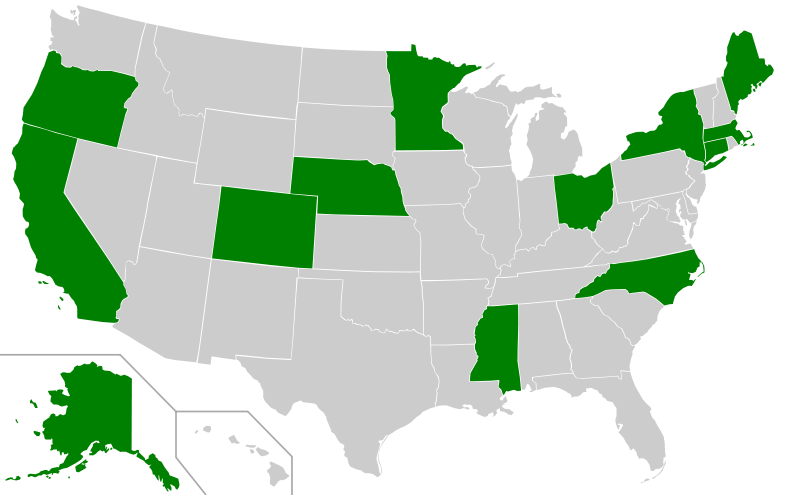
\includegraphics[width=0.6\textwidth]{images/hashmap.png}\\
		\hspace*{15pt}\hbox{\scriptsize Image By:\thinspace{\itshape Photohound}}
	\end{center}
\end{frame}

\begin{frame}
	\frametitle{Hashmaps}
		\begin{block}{Hashmaps}
			Implement the Map ADT using Hash tables.\\
			\pause
			With a good hash function, we expect: $\Theta(1)$ insertion/deletion/retrieval.\\
			But worst-case they are still $\Theta(n)$.
		\end{block}	
		\pause
		\begin{block}{Handling hashing conflicts}
			Different options to handle hash conflicts:
			\begin{itemize}
				\item Separate Chaining
				\item (Linear) Probing
			\end{itemize}
		\end{block}
\end{frame}

\begin{frame}
	\frametitle{Lets start with the basics}
	\vspace{-13pt}
	\begin{columns}
		\column{0.355\textwidth}
		\begin{itemize}
			\item Creating a new hashmap
			\item<2-> Getting the size
			\item<3-> A hash function for keys in this map
			\item<4-> Getting an item
			\item<4-> Putting an item
		\end{itemize}
		\column{0.555\textwidth}
			
		\lstinputlisting[basicstyle=\tiny\ttfamily
		% ,linebackgroundcolor={%
			% \btLstHL<1>{3-5}%
			% \btLstHL<2>{7-8}%
			% \btLstHL<3>{10-11}%
			% \btLstHL<4>{13-15}%
			% \btLstHL<5>{17-21}%
		% }
		]
		{src/hashmap.py}
	\end{columns}
	\only<5->{
			\begin{block}{So conclusion}
				It depends on how we put things into the buckets!\\
				Do we use the linked list? Or do we do something else?
			\end{block}	
	}
\end{frame}


\begin{frame}
	\frametitle{Recap of Maps}
	
	\begin{center}
		\begin{tabular}{c | c | c}
			Operation & Expected Time & Worst-case \\
			\midrule
			\texttt{M.size()} & $\Theta(1)$& $\Theta(1)$\\
			\texttt{M.get(k)}  & $\Theta(1)$& $\Theta(n)$\\
			\texttt{M.put(k,v)} & $\Theta(1)$& $\Theta(n)$\\
			\texttt{M.remove(k)} & $\Theta(1)$& $\Theta(n)$\\
			\texttt{M.contains(k)} & $\Theta(1)$& $\Theta(n)$\\
		\end{tabular}
	\end{center}
		\begin{block}{What does this depend on?}
			It all stands or falls with the hash function!
			\begin{itemize}
				\item Fewer hash-conflicts means better performance.
				\item Separate chaining or (linear) probing does not matter for time performance.
				\item The latter saves us some space, but is not better in terms of space or time \textit{complexity}.
			\end{itemize}
		\end{block}	
\end{frame}



%%%%%%%%%%%%%%%%%%%%%%%%%%%%%%%%%%%%%%%%%%%%%%%%%%%%%%%%%%%%%%%%%%%%%%
\begin{frame}[fragile]\frametitle{}
\begin{center}
{\Large Trees}
\end{center}

\end{frame}


\begin{frame}
	\frametitle{Binary Trees}
	\framesubtitle{Tikz taken from: \url{http://texample.net/tikz/examples/red-black-tree/}}
	\begin{center}
			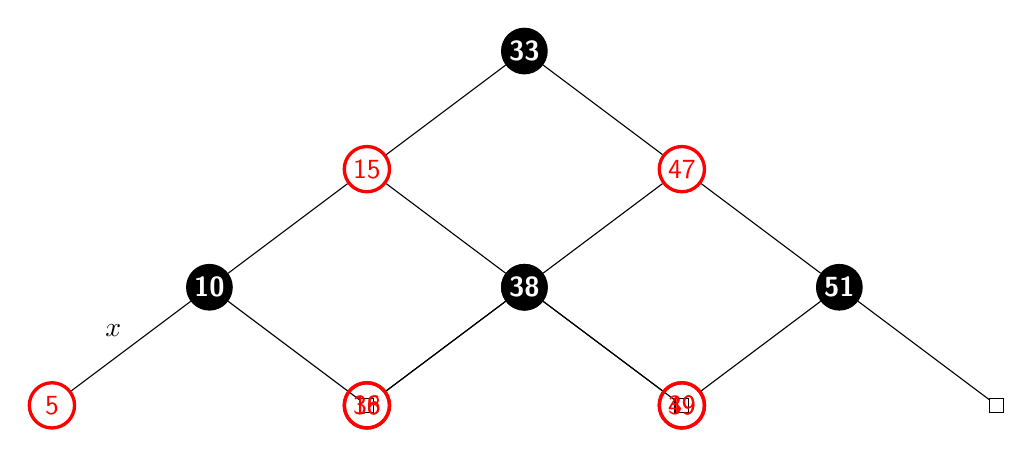
\begin{tikzpicture}[level/.style={sibling distance = 4cm, %->,>=stealth',
		  level distance = 1.5cm},
			  treenode/.style = {align=center, inner sep=0pt, text centered,
		    font=\sffamily},
		  arn_n/.style = {treenode, circle, white, font=\sffamily\bfseries, draw=black,
		    fill=black, text width=1.5em},% arbre rouge noir, noeud noir
		  arn_r/.style = {treenode, circle, red, draw=red,
		    text width=1.5em, very thick},% arbre rouge noir, noeud rouge
		  arn_x/.style = {treenode, rectangle, draw=black,
		    minimum width=0.5em, minimum height=0.5em}% arbre rouge noir, nil
			]
			\node [arn_n] {33}
    child{ node [arn_r] {15}
            child{ node [arn_n] {10}
            	child{ node [arn_r] {5} edge from parent node[above left]
                         {$x$}} %for a named pointer
							child{ node [arn_x] {}}
            }
            child{ node [arn_n] {20}
							child{ node [arn_r] {18}}
							child{ node [arn_x] {}}
            }
    }
    child{ node [arn_r] {47}
            child{ node [arn_n] {38}
							child{ node [arn_r] {36}}
							child{ node [arn_r] {39}}
            }
            child{ node [arn_n] {51}
							child{ node [arn_r] {49}}
							child{ node [arn_x] {}}
            }
		}
;
\end{tikzpicture}
	\end{center}
	
\end{frame}

\begin{frame}
	\frametitle{Binary Trees}
	\framesubtitle{All we need}

		\begin{block}{Binary Trees}
			\begin{itemize}
				\item Every node has at most 2 children.
					\pause
				\item One \textit{left} child and one \textit{right} child.
			\end{itemize}
		\pause
		A binary tree is \textit{proper} or \textit{full} if all nodes have either 0 or 2 children.
		\end{block}	

		\pause
		\begin{columns}
			\column{0.455\textwidth}
				
			\begin{tikzpicture}[
				level distance = 2.5em,
				level 1/.style={sibling distance=9em},
				level 2/.style={sibling distance=4.5em},
				level 3/.style={sibling distance=2.25em},
			]
			\node[circle] (t1) {root}
				child { node[circle]   {child 1}
					child { node[circle] {l1}}
					child { node[circle] {l2}}
				}
				child { node[circle]   {child 2}
					child { node[circle] {l3}}
					child { node[circle] {l4}
						child { node[circle] {l5}}
						child { node[circle] {l6}}
					}
				};
			\end{tikzpicture}
			\column{0.455\textwidth}
				
			\begin{block}{Is it full?}
				Is this tree full?
				\begin{enumerate}[A.]
					\item Yes
					\item No
					\item I don't know
				\end{enumerate}
			\end{block}
		\end{columns}
\end{frame}

\begin{frame}
	\frametitle{All kinds of fun properties!}
	
		\begin{block}{Many interesting properties}
			There are many interesting relations in binary trees, between the number of internal nodes vs leaves, height, etc.	
		\end{block}	
		\pause
		\begin{block}{Just one example}
			There is always one more leaf than there are internal nodes in a full binary tree.
		\end{block}	
\end{frame}

\begin{frame}
	\frametitle{Tree properties pt2}
	\begin{center}
		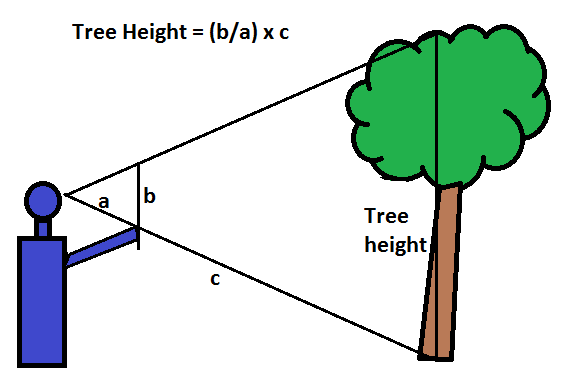
\includegraphics[width=0.6\textwidth]{images/stick.png}\\
		\hspace*{15pt}\hbox{\scriptsize Image By:\thinspace{\itshape Edfrank01}}
		% https://commons.wikimedia.org/wiki/File:Stick_measurement.png
	\end{center}
\end{frame}

\begin{frame}
	\frametitle{Depth of a node}

	\begin{columns}
		\column{0.405\textwidth}
			\begin{tikzpicture}[
				level distance = 2.5em,
				level 1/.style={sibling distance=9em},
				level 2/.style={sibling distance=4.5em},
				level 3/.style={sibling distance=2.25em},
			]
			\node[circle] (t1) {root}
				child { node[circle]   {child 1}
					child { node[circle] {l1}}
				}
				child { node[circle]   {child 2}
					child { node[circle] {l2}}
					child { node[circle] {l3}}
					child { node[circle] {l4}}
				};
			\end{tikzpicture}
		\column{0.555\textwidth}
		\begin{itemize}
			\item The \textit{depth} of a \alert<5->{node} is the distance to the root.
				\pause
			\item So depth(root) = 0.
			\item And depth(l2) = 2.
				\pause
			\item The \textit{height} of a \alert<5->{tree} is the length of the longest path from root to leaf.
				\pause
			\item So the height of this tree is 3.
				\pause
			\item Note: Every book/author has their own definition of these things! Including our book :(
		\end{itemize}
	\end{columns}
	
\end{frame}

\begin{frame}
	\frametitle{Depth of a node}

	\begin{columns}
		\column{0.405\textwidth}
			\begin{tikzpicture}[
				level distance = 2.5em,
				level 1/.style={sibling distance=9em},
				level 2/.style={sibling distance=4.5em},
				level 3/.style={sibling distance=2.25em},
			]
			\node[circle] (t1) {root}
				child { node[circle]   {child 1}
					child { node[circle] {l1}}
				}
				child { node[circle]   {child 2}
					child { node[circle] {l2}}
					child { node[circle] {l3}}
					child { node[circle] {l4}}
				};
			\end{tikzpicture}
		\column{0.555\textwidth}
		\begin{block}{Alternative definition for height}
			How can we also describe the tree height of a tree $T$?
			\pause
			\begin{enumerate}[A.]
				\item $\max\limits_{v\in T}({\textit{depth}(v)})-1$
				\item $\max\limits_{v\in T}({\textit{depth}(v)})$
				\item $\max\limits_{v\in T}({\textit{depth}(v)})+1$
			\end{enumerate}
		\end{block}
	\end{columns}
	\pause
	\begin{block}{A tree of height one}
		Remember that a tree of height one is just the root, which is at depth $0$. So it cannot be A or B.\\
		Then remember that depth is the distance, but height is the length of the path. These differ by 1, so C is the right
		answer.\\
		Our book uses $B$ :( 
	\end{block}
\end{frame}

\begin{frame}
	\frametitle{An implementation}
	
	\begin{block}{How do we implement this?}
		How can we implement such a tree structure?
	\end{block}
	\pause
	\begin{block}{Just like a DLL, only different}
		By using nodes that are \textit{linked} together to form a tree!
	\end{block}
	\pause
	\begin{columns}[t]
		\column{0.535\textwidth}
	\lstinputlisting{src/tree.py}
			
		\column{0.505\textwidth}
	\lstinputlisting{src/treenode.py}
			
	\end{columns}
\end{frame}

\begin{frame}
	\frametitle{Now we can create functions!}
	\begin{block}{Implementing functionality}
		What kind of \textit{programming paradigm} will we use to implement tree functions?
	\end{block}
	\pause
	\begin{block}{See the contents of this box}
		See the title of this box.
	\end{block}
\end{frame}

\begin{frame}
	\frametitle{Node Depth}
		\begin{block}{Example: Node depth}
			Find the depth of a node is easy if we know the depth of the parent.
		\end{block}	
		\pause
		\lstinputlisting{src/nodedepth.py}
\end{frame}

\begin{frame}
	\frametitle{Tree Height}
		\begin{block}{Example: Tree height}
			The height of the tree is the max depth + 1! 	
		\end{block}	
		\pause
		\lstinputlisting{src/treeheight.py}
\end{frame}

\begin{frame}
	\frametitle{Getting all the leaves}
	\begin{block}{It's autumn time}
		How can we get all the leaves from a tree?
	\end{block}
		\pause
		\lstinputlisting{src/treeleaves.py}
\end{frame}

\begin{frame}
	\frametitle{The full ADT}
		\begin{block}{A Tree ADT}
			Different implementations of trees, give you different ADTs.\\
			The book uses one which is \textit{position}-focused.\\
			The properties are always the same, just the functions and how to call them can be different.
		\end{block}	
\end{frame}

\begin{frame}
	\frametitle{Alternative implementation}
		\begin{block}{An observation}
			Every node in a tree, is the root to a subtree!
		\end{block}	
		\pause
		\begin{columns}
			\column{0.455\textwidth}
				
			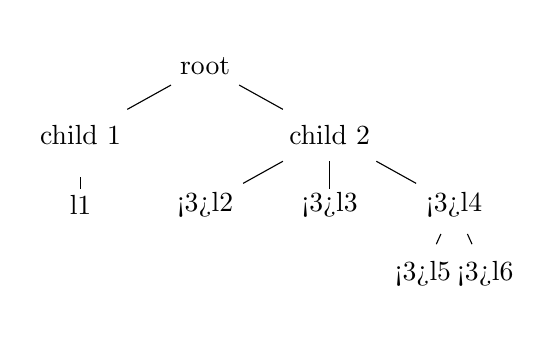
\begin{tikzpicture}[
				level distance = 2.5em,
				level 1/.style={sibling distance=9em},
				level 2/.style={sibling distance=4.5em},
				level 3/.style={sibling distance=2.25em},
			]
			\node[circle] (t1) {root}
				child { node[circle]   {child 1}
					child { node[circle] {l1}}
				}
				child { node[circle]   {child 2} % ,
					child { node[circle] {\alert<3>{l2}}}
					child { node[circle] {\alert<3>{l3}}}
					child { node[circle] {\alert<3>{l4}}
						child { node[circle] {\alert<3>{l5}}}
						child { node[circle] {\alert<3>{l6}}}
					}
				};
			\end{tikzpicture}
			\pause
			\column{0.455\textwidth}
				\begin{block}{A subtree}
					In the example on the right, child 2 is the root of the subtree drawn in red.
				\end{block}	
		\end{columns}
\end{frame}

\begin{frame}
	\frametitle{Alternative implementation}
		\begin{block}{Thinking of all nodes as trees}
			By implementing it like this, we have no need for \texttt{TreeNode}s. All nodes are just \texttt{Tree}s!
		\end{block}	

		\lstinputlisting{src/tree_alt.py}
\end{frame}

\begin{frame}
	\frametitle{Alternative implementation: Tree Height}
	\begin{block}{What do we do?}
		How do we determine the height in this set-up?
	\end{block}
	\pause
	\lstinputlisting{src/tree_alt_height.py}
\end{frame}

\begin{frame}
	\frametitle{Why have one implementation over the other?}

	\begin{block}{Which is better?}
		Which implementation should you use?
	\end{block}
	\pause
	\begin{block}{IT DEEP ENDS}
		It depends of course ;)\\
		What information do you need to store for your use case?
	\end{block}
	
\end{frame}



\begin{frame}
	\frametitle{Tree time}
	\begin{center}
		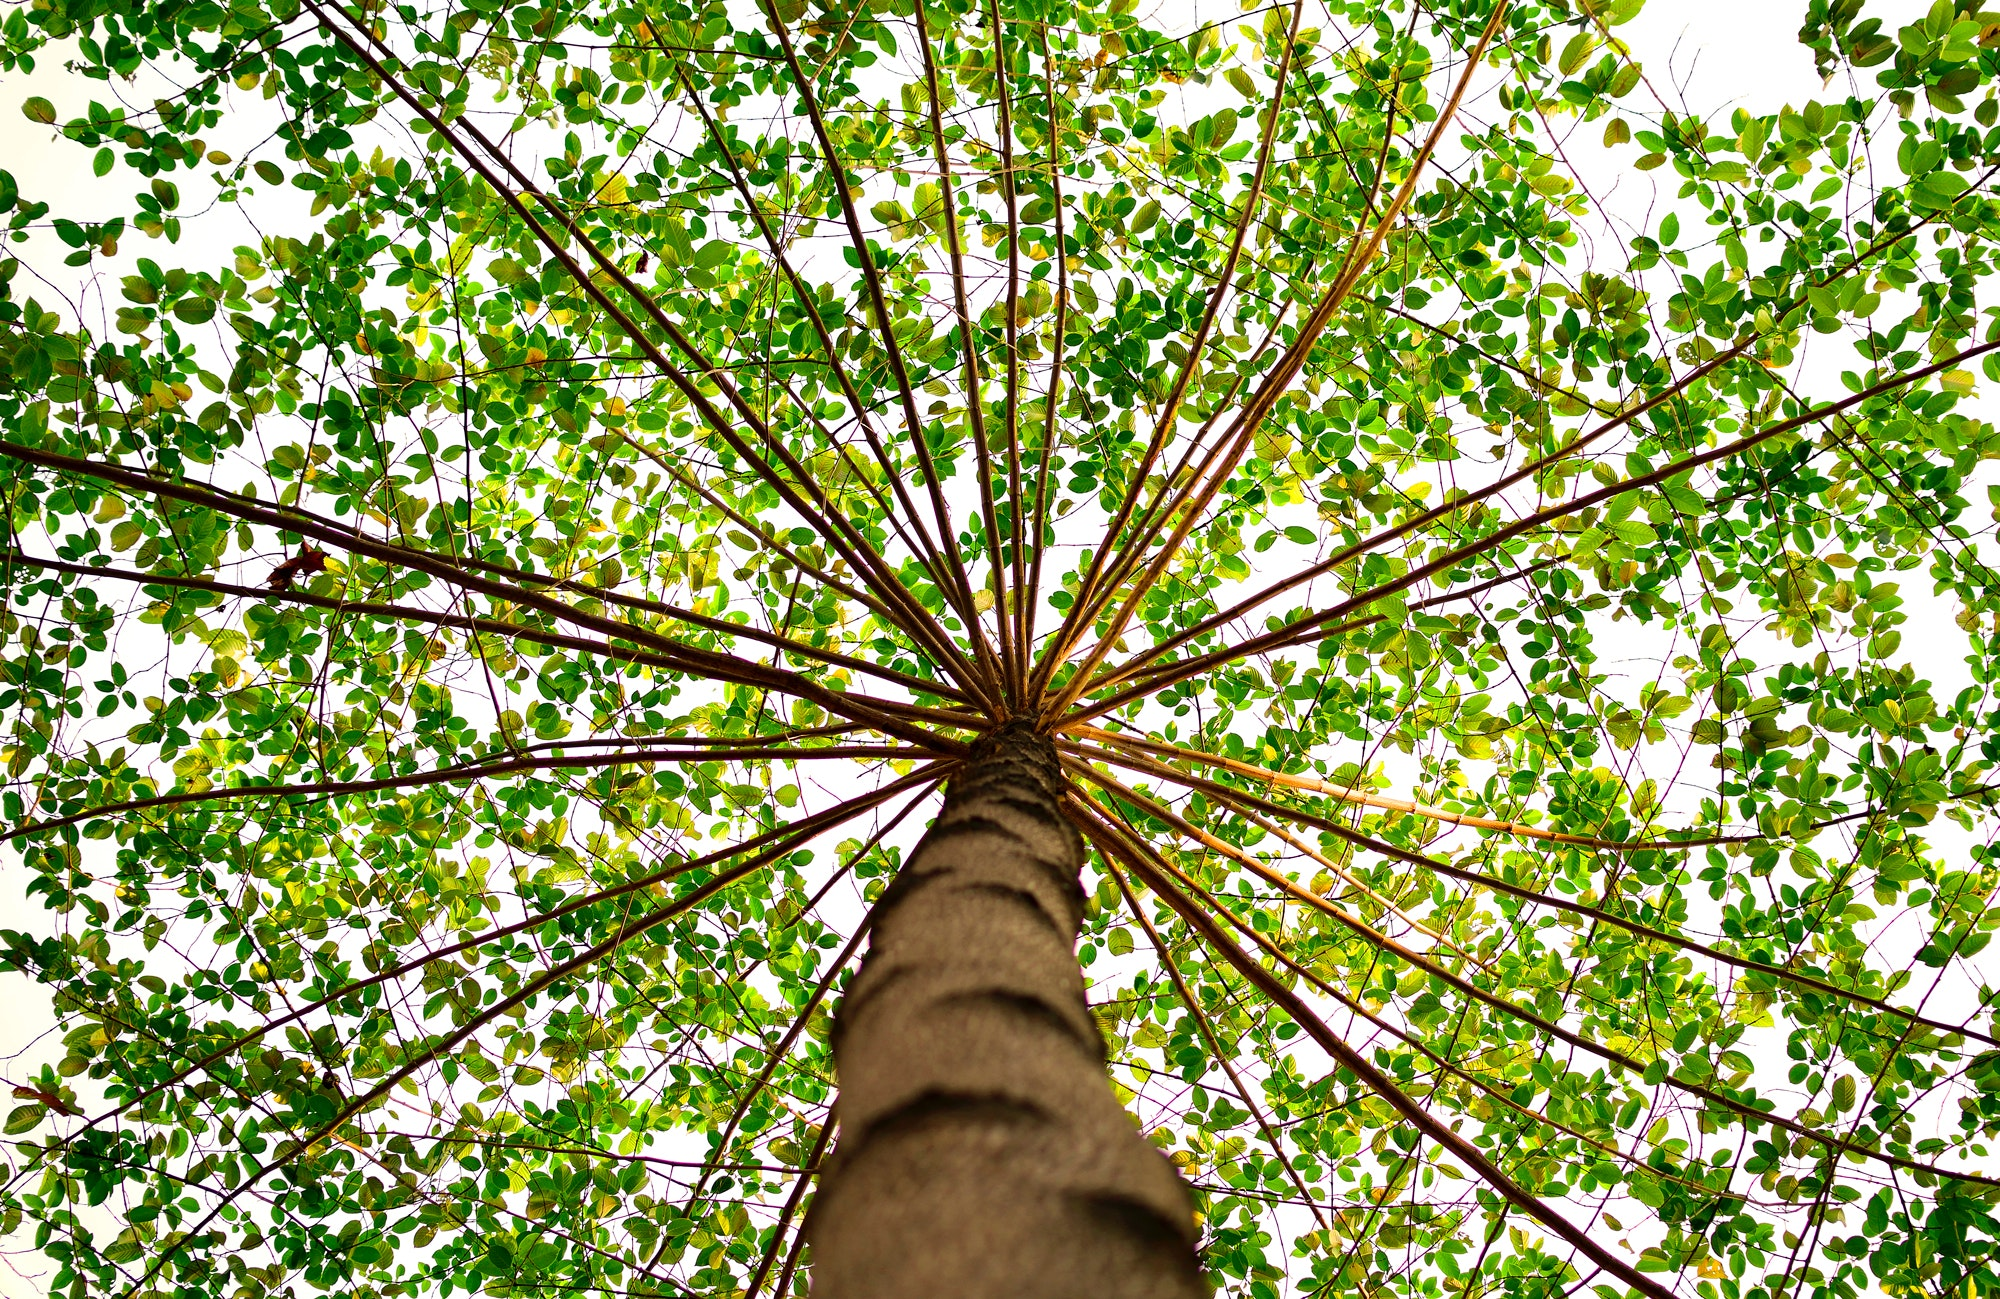
\includegraphics[width=0.6\textwidth]{images/tree.jpg}\\
		\hspace*{15pt}\hbox{\scriptsize Image By:\thinspace{\itshape George achik}}
		% https://commons.wikimedia.org/wiki/File:Last_summer_time_tree_and_evening_time,_In_Srimongol,_Bangladesh.jpg
	\end{center}
\end{frame}

\begin{frame}
	\frametitle{Properties}
	\begin{columns}
		\column{0.405\textwidth}
			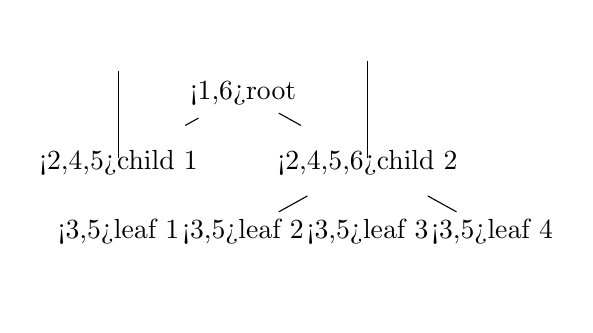
\begin{tikzpicture}[
				level distance = 2.5em,
				level 1/.style={sibling distance=9em},
				level 2/.style={sibling distance=4.5em},
				level 3/.style={sibling distance=2.25em},
			]
			\node[circle] (t1) {\alert<1,6>{root}} % ,onslide=<5>{draw=red}
				child { node[circle] {\alert<2,4,5>{child 1}}
					child { node[circle] {\alert<3,5>{leaf 1}}}
				}
				child { node[circle] {\alert<2,4,5,6>{child 2}}
					child { node[circle] {\alert<3,5>{leaf 2}}}
					child { node[circle] {\alert<3,5>{leaf 3}}}
					child { node[circle] {\alert<3,5>{leaf 4}}}
				};
			\end{tikzpicture}
		\column{0.555\textwidth}
		\begin{itemize}
			\item The \textit{root node} is the node that has no \textit{parent}.
				\pause
			\item A node can have \textit{children}.
				\pause
			\item A node without children is called a \textit{leaf}.
				\pause
			\item Two nodes with the same \textit{parent} are \textit{siblings}.
				\pause
			\item \textit{Descendants} are found by repeatedly following child-relations.
				\pause
			\item \textit{Ancestors} are found by repeatedly following parent-relations.
		\end{itemize}
	\end{columns}
\end{frame}

\begin{frame}
	\frametitle{Quick check}
	
	\begin{columns}
		\column{0.405\textwidth}
			\begin{tikzpicture}[
				level distance = 2.5em,
				level 1/.style={sibling distance=2em},
				level 2/.style={sibling distance=4.5em},
				level 3/.style={sibling distance=2.25em},
			]
			\node[circle] (t1) {r}
				child { node[circle] {k}
					child { node[circle] {d}}
				}
				child { node[circle] {a} }
				child { node[circle] {b} }
				child { node[circle] {e} 
					child { node[circle] {g} }
					child { node[circle] {h}
						child { node[circle] {i}}
					}
				}
				child { node[circle] {f} };
			\end{tikzpicture}
		\column{0.555\textwidth}
		\pause
			\begin{block}{Let's see if that was a clear}
				Let $c(v)$ be the set of children of $v$.\\
				Let $d(v)$ be the set of descendants of $v$.\\
				Let $s(v)$ be the set of siblings of $v$.\\
				Let $a(v)$ be the set of ancestors of $v$.\\
				Let $p(v)$ be the parent of $v$.\\
				What is: $|c(k)| + |d(p(g))| + \sum\limits_{v \in a(h)} |s(v)|$?
				% \begin{multicols}{2}
				\begin{enumerate}[A.]
					\item 4
					\item 8
					\item 12
					\item I don't know
				\end{enumerate}
			% \end{multicols}
			\end{block}
	\end{columns}
	\pause
	\vspace{-5pt}
	\begin{block}{Arithmetic time}
		$c(k) = \{d\}$, $p(g) = e$, $d(e) = \{g,h,i\}$, $a(h) = \{r,e\}$, $s(r) = \emptyset$, $s(e) = \{k,a,b,f\}$. So the
		final answer is: $1+3+4=8$.
	\end{block}
\end{frame}


\begin{frame}
	\frametitle{Tree traversals}
	\framesubtitle{Walking through our tree}

	\begin{center}
		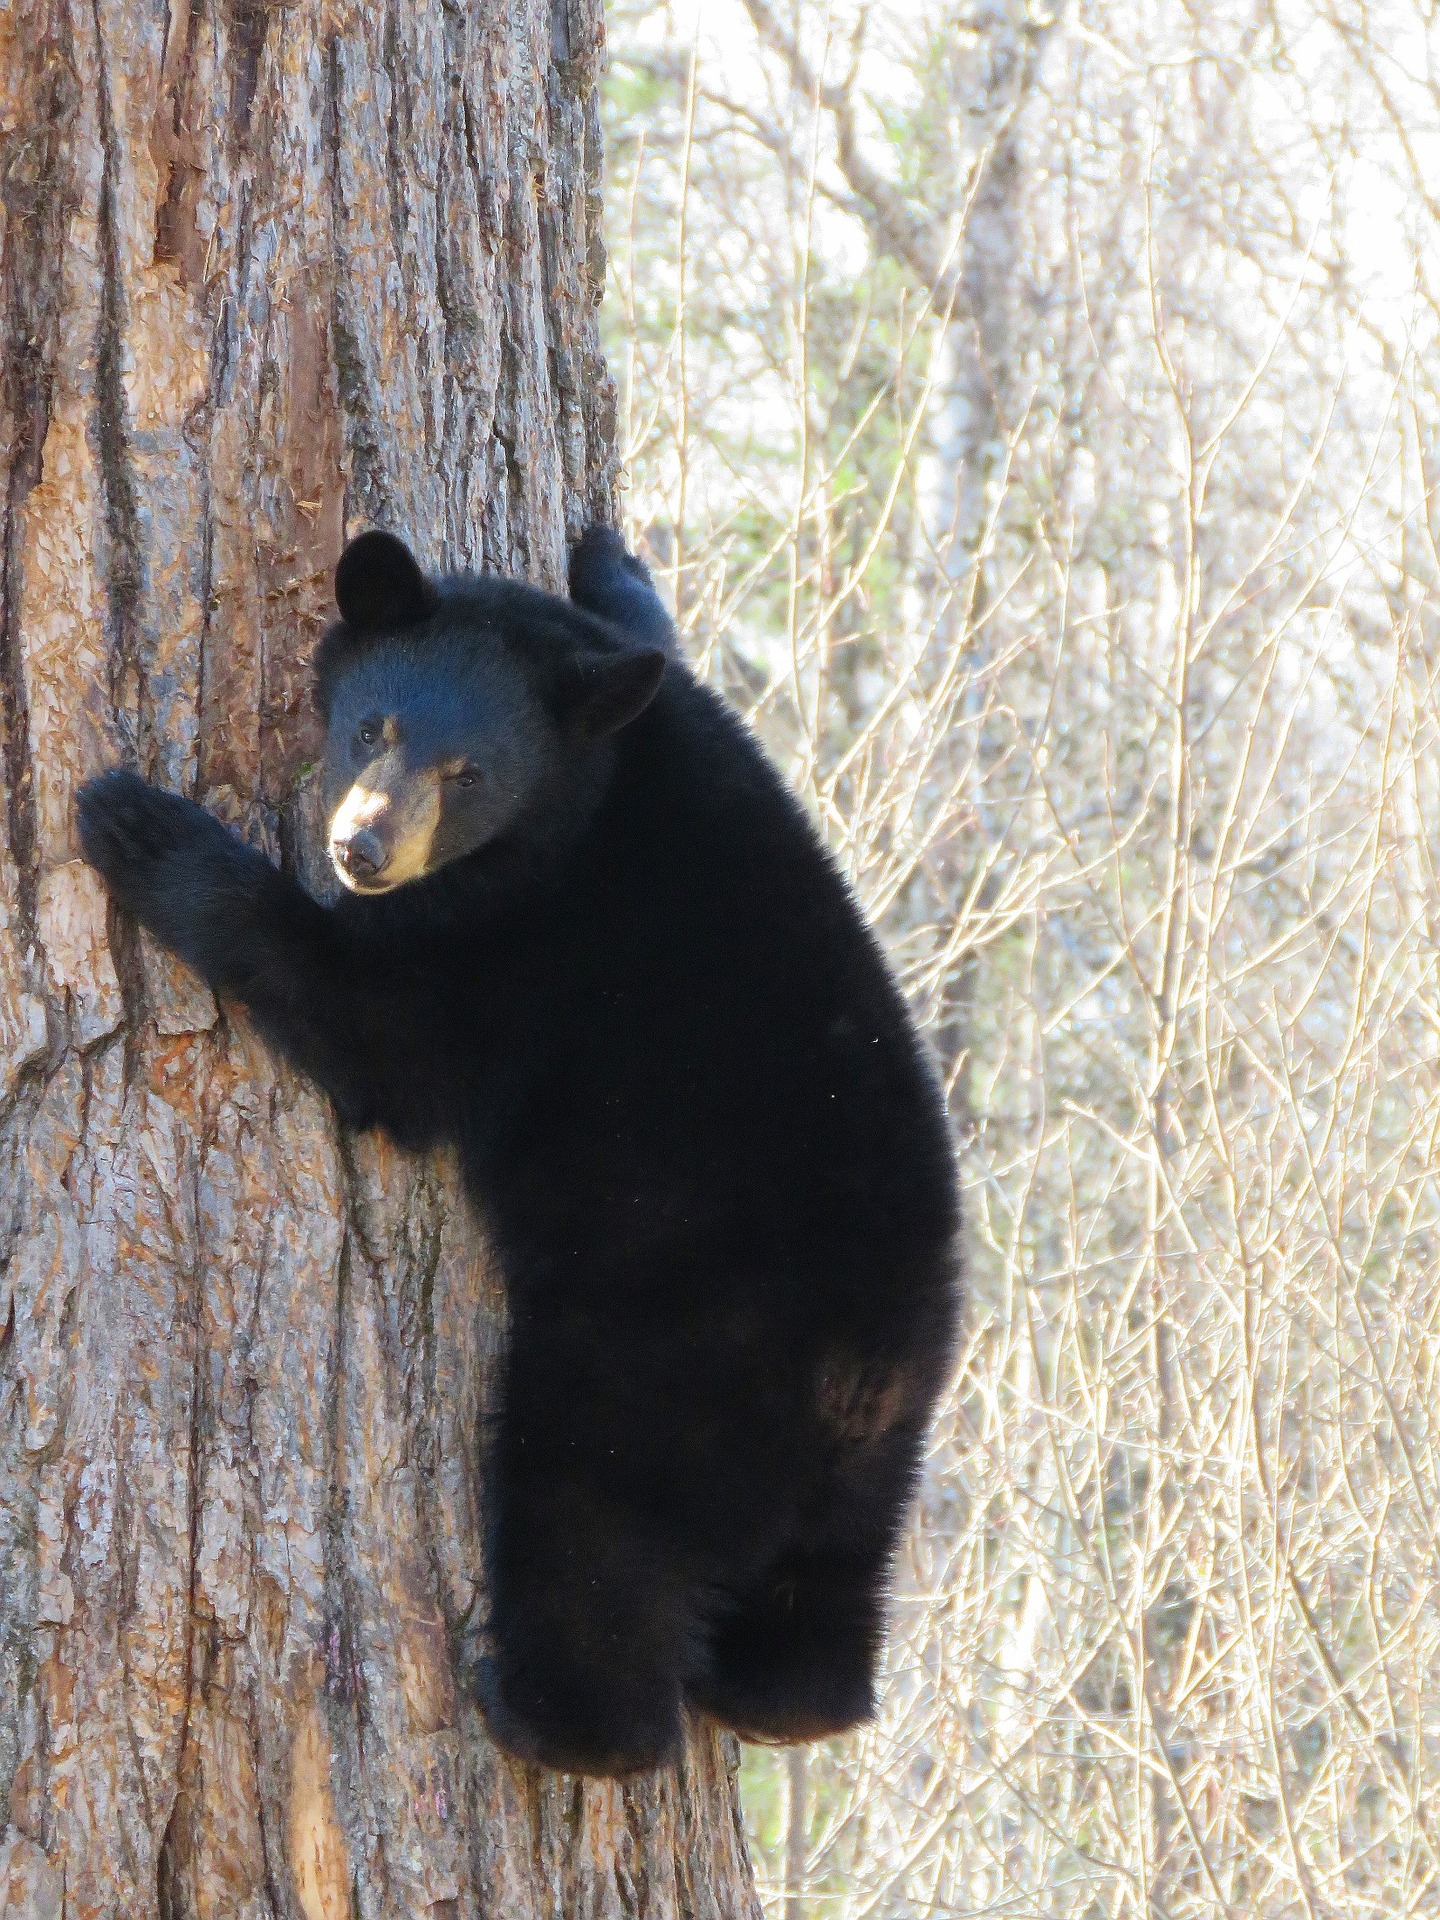
\includegraphics[trim={0 4cm 0 4cm},clip, width=0.65\textwidth]{images/bearcub.jpg}\\
		\hspace*{15pt}\hbox{\scriptsize Image By:\thinspace{\itshape Skeeze}}
		% https://pixabay.com/photos/bear-cub-brown-climbing-tree-1576559/
	\end{center}

\end{frame}

\begin{frame}
	\frametitle{Iterating over the nodes}
	
		\begin{block}{Finding all the nodes}
			If you want to iterate over the tree, you can do so in many different orders. Three common ones for binary trees are:
			\begin{itemize}
				\item Pre-order traversal
				\item In-order traversal
				\item Post-order traversal
			\end{itemize}
		\end{block}	
\end{frame}

\begin{frame}
	\frametitle{Pre-order traversal}
	\begin{overlayarea}{\textwidth}{\textheight}
			\begin{columns}
				\column{0.455\textwidth}
				\begin{itemize}
					\item First give the value of the current node.
					\item Then a pre-order traversal of the left child.
					\item Then a pre-order traversal of the right child.
				\end{itemize}
				\column{0.455\textwidth}
				\pause
					\begin{tikzpicture}[
						level distance = 2.5em,
						level 1/.style={sibling distance=9em},
						level 2/.style={sibling distance=4.5em},
						level 3/.style={sibling distance=2.25em},
					]
					\node[circle] (t1) {\alert<3>{1}}
					child { node[circle]   {\alert<4>{2}}
						child { node[circle] {\alert<5>{3}}}
						}
						child { node[circle]   {\alert<6>{4}}
							child { node[circle] {\alert<7>{5}}}
							child { node[circle] {\alert<8>{6}}
								child { node[circle] {\alert<9>{7}}}
								child { node[circle] {\alert<10>{8}}}
							}
						};
					\end{tikzpicture}
			\end{columns}
			\only<11>{
			\begin{block}{Amsterdam, Rotterdam, no not that kind of topology!}
				Gives us a \textit{topological} order of the tree.\\
				If all nodes represent jobs, and job $i$ depends on it's parent job $p$ then this gives us an order in which we can
				do all jobs, satisfying these dependencies.
			\end{block}
		}
	\end{overlayarea}
\end{frame}

\begin{frame}
	\frametitle{In-order traversal}
	\begin{overlayarea}{\textwidth}{\textheight}
			\begin{columns}
				\column{0.455\textwidth}
				\begin{itemize}
					\item First an in-order traversal of the left child.
					\item Then give the value of the current node.
					\item Then an in-order traversal of the right child.
				\end{itemize}
				\column{0.455\textwidth}
					\begin{tikzpicture}[
						level distance = 2.5em,
						level 1/.style={sibling distance=9em},
						level 2/.style={sibling distance=4.5em},
						level 3/.style={sibling distance=2.25em},
					]
					\node[circle] (t1) {\alert<5>{1}}
					child { node[circle]   {\alert<4>{2}}
						child { node[circle] {\alert<3>{3}}}
						}
						child { node[circle]   {\alert<7>{4}}
							child { node[circle] {\alert<6>{5}}}
							child { node[circle] {\alert<9>{6}}
								child { node[circle] {\alert<8>{7}}}
								child { node[circle] {\alert<10>{8}}}
							}
						};
					\end{tikzpicture}
			\end{columns}
			\only<2>{
				\begin{block}{In-order}
				What is the order of nodes now?
				% \begin{multicols}{2}
					\begin{enumerate}[A.]
						\item 1,2,3,4,5,6,7,8
						\item 3,2,1,5,4,7,6,8
						\item 3,2,8,7,6,5,4,1
						\item 8,7,6,5,4,3,2,1
					\end{enumerate}
				% \end{multicols}
			\end{block}
		}
			\only<11>{
				\begin{block}{We'll save that for tomorrow}
				We will see an example for this tomrrow!
			\end{block}
		}
	\end{overlayarea}
\end{frame}

\begin{frame}
	\frametitle{Post-order traversal}
	\begin{overlayarea}{\textwidth}{\textheight}
			\begin{columns}
				\column{0.455\textwidth}
				\begin{itemize}
					\item First a post-order traversal of the left child.
					\item Then a post-order traversal of the right child.
					\item Then give the value of the current node.
				\end{itemize}
				\column{0.455\textwidth}
					\begin{tikzpicture}[
						level distance = 2.5em,
						level 1/.style={sibling distance=9em},
						level 2/.style={sibling distance=4.5em},
						level 3/.style={sibling distance=2.25em},
					]
					\node[circle] (t1) {\alert<10>{1}}
					child { node[circle]   {\alert<4>{2}}
						child { node[circle] {\alert<3>{3}}}
						}
						child { node[circle]   {\alert<9>{4}}
							child { node[circle] {\alert<5>{5}}}
							child { node[circle] {\alert<8>{6}}
								child { node[circle] {\alert<6>{7}}}
								child { node[circle] {\alert<7>{8}}}
							}
						};
					\end{tikzpicture}
			\end{columns}
			\only<2>{
				\begin{block}{Post-order}
				What is the order of nodes now?
				% \begin{multicols}{2}
					\begin{enumerate}[A.]
						\item 1,2,3,4,5,6,7,8
						\item 3,2,5,8,7,6,4,1
						\item 3,2,8,7,6,5,4,1
						\item 8,7,6,5,4,3,2,1
					\end{enumerate}
				% \end{multicols}
			\end{block}
		}
			\only<11>{
				\begin{block}{I didn't mean to sound so dark :(}
				Used to delete a tree (first delete your children, before deleting yourself).
			\end{block}
		}
	\end{overlayarea}
\end{frame}

\begin{frame}
	\frametitle{It's all about balance}
	\begin{center}
		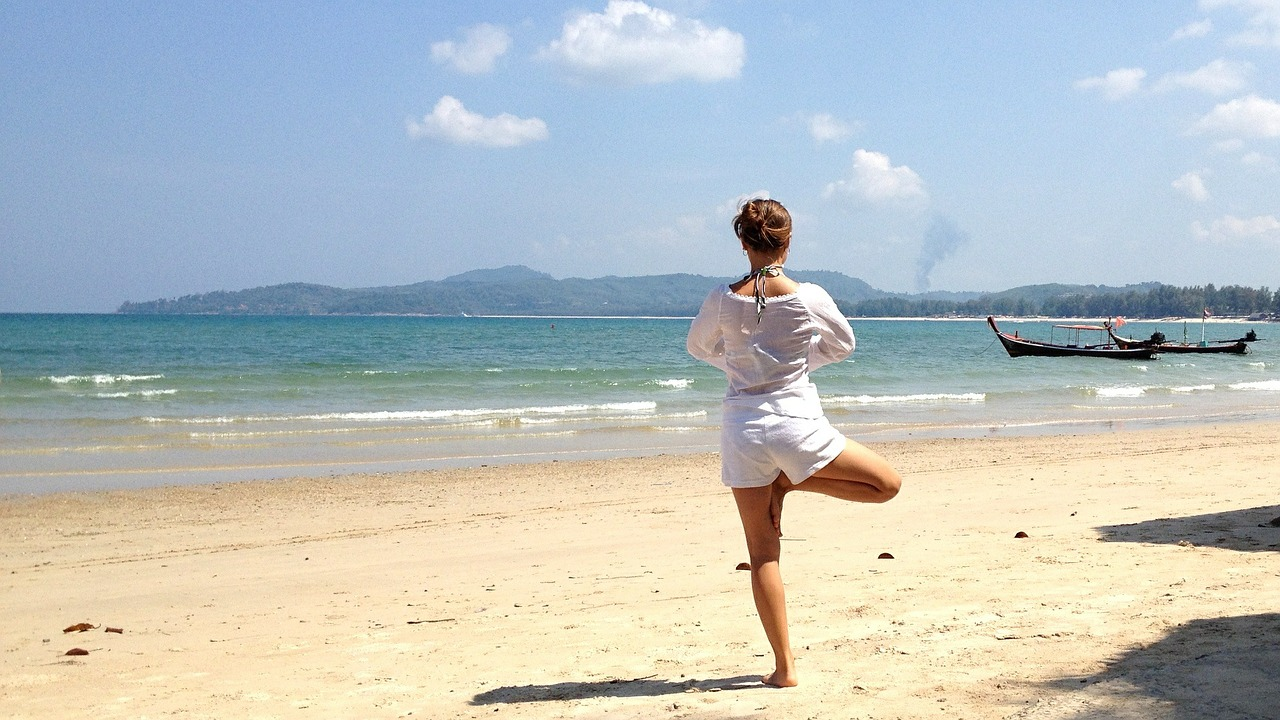
\includegraphics[width=0.8\textwidth]{images/balance.jpg}\\
		\hspace*{15pt}\hbox{\scriptsize Image By:\thinspace{\itshape Evitaochel}}
		% https://pixabay.com/photos/balance-yoga-zen-exercise-405513/
	\end{center}
\end{frame}

\begin{frame}
	\frametitle{Limiting the height}
	\begin{block}{The idea}
		If we can somehow limit the height to be $\Theta(\log n)$ we are all set.
	\end{block}	
	\pause
	This is where the tens of options come in...
	\begin{itemize}
		\item AVL-trees
		\item Red-Black trees
		\item Splay-trees
		\item And many more\dots
	\end{itemize}
\end{frame}

\begin{frame}
	\frametitle{AVL-Trees}
	\framesubtitle{Named after Adel'son-Vel'skii and Landis}

		\begin{block}{AVL-trees}
			It is a binary search tree, with one more constraint:\\
			The height of the left-subtree and right-subtree of a node differ by at most 1 for all nodes in the tree.
		\end{block}	

	\begin{columns}
		\column{0.455\textwidth}

		\begin{tikzpicture}[
			level distance = 2.5em,
			level 1/.style={sibling distance=9em},
			level 2/.style={sibling distance=4.5em},
			level 3/.style={sibling distance=2.25em},
			]
			\node[circle] (t1) {12}
			child { node[circle]   {3}
				child[draw=white] { }
				child { node[circle] {9}}
			}
			child { node[circle]   {25}
				child { node[circle] {14}}
				child { node[circle] {29}
					child { node[circle] {26}}
					child { node[circle] {32}}
				}
			};
		\end{tikzpicture}
		\column{0.455\textwidth}

		\begin{block}{Is it full?}
			Is this tree an AVL-tree?
		\end{block}
		\pause
		\begin{block}{}
			Yes :)	
		\end{block}
	\end{columns}
\end{frame}

\begin{frame}
	\frametitle{AVL-trees}
	\begin{block}{Height}
		This guarantees the height to be $\Theta(\log n)$ (check the book for a proof if you want).
	\end{block}

	\pause
	\begin{block}{Inserting/deleting nodes}
		How do we now insert or delete nodes from this AVL tree?
	\end{block}
\end{frame}

\begin{frame}
	\frametitle{Inserting items}

	\begin{block}{Observations}
		\begin{itemize}
			\item If we insert like we did in a ``regular'' binary search tree\dots
			\item Then we only upset (potentially) the ancestors of the node where we insert it.
				\pause
			\item Let's look at an example ;)
		\end{itemize}
	\end{block}	
	\pause
	\begin{block}{Inserting an item}
		\begin{columns}
			\column{0.455\textwidth}

			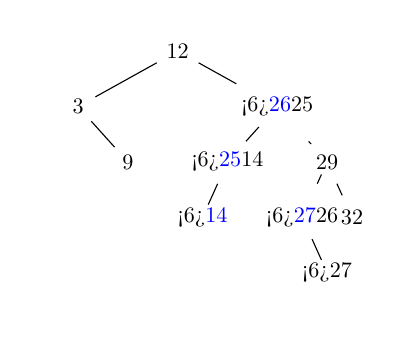
\begin{tikzpicture}[
				level distance = 2.5em,
				level 1/.style={sibling distance=9em},
				level 2/.style={sibling distance=4.5em},
				level 3/.style={sibling distance=2.25em},
				scale=0.8,transform shape
				]
				\node[circle] (t1) {12}
				child { node[circle]   {3}
					child[draw=white] { }
					child { node[circle] {9}}
				}
				child { node[circle]   {\alt<6>{\color{blue}26}{25}}
					child { node[circle] {\alt<6>{\color{blue}{25}}{14}}
						child[] { node[circle] {\alt<6>{\color{blue}{14}}{}}}
						child[draw=white] { }
					}
					child { node[circle] {29}
						child { node[circle] {\alt<6>{\color{blue}27}{26}}
							child[draw=white] { }
							child[] { node[circle] {\alt<6>{}{27}}}
						}
						child { node[circle] {32}}
					}
				};
			\end{tikzpicture}
			\column{0.455\textwidth}
			\begin{itemize}
				\item Two items are now upsetting the AVL-property.
					\pause
				\item So we need to fix that!
					\pause
				\item We can do so by \textit{rotating} some nodes around.
					\pause
				\item To end up with this.
			\end{itemize}
		\end{columns}
	\end{block}	
\end{frame}

\begin{frame}
	\frametitle{A tri-node restructering}
	\framesubtitle{Draw this for yourself!}
	\vspace{-15pt}
	\begin{columns}
		\column{0.455\textwidth}
			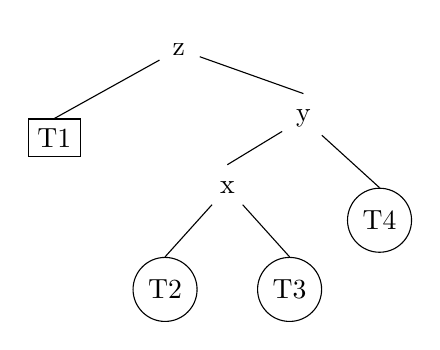
\begin{tikzpicture}[
				level distance = 2.5em,
				level 1/.style={sibling distance=9em},
				level 2/.style={sibling distance=5.5em},
				level 3/.style={sibling distance=4.5em},
				child anchor =north
				]
				\node[circle] (t1) {z}
				child { node[draw=black, anchor = north]   {T1}
				}
				child { node[circle]   {y}
					child { node[circle] {x}
						child { node[circle, anchor = north, draw=black] {T2}}
						child { node[circle, anchor = north, draw=black] {T3}}
					}
					child { node[circle, anchor = north, draw=black] {T4}
					}
				};
			\end{tikzpicture}
		\column{0.455\textwidth}
		\begin{itemize}
			\item This is the situation before inserting (we chose these heights to make the insertion interesting).
				\pause
				\begin{itemize}
					\item $z$ has a height of $h+2$
					\item $y$ has a height of $h+1$
					\item $x$ has a height of $h$
					\item $T1,T4$ have a height of $h$
					\item $T2,T3$ have a height of $h-1$
				\end{itemize}
				\pause
			\item We now insert an item into T3, which causes an imbalance in node z.
				\pause
				\begin{itemize}
					\item $z$ has a height of $h+3$
					\item $y$ has a height of $h+2$
					\item $x$ has a height of $h+1$
					\item $T1,T3,T4$ have a height of $h$
					\item $T2$ has a height of $h-1$
				\end{itemize}
		\end{itemize}
			
	\end{columns}
\end{frame}

\begin{frame}
	\frametitle{A tri-node restructering}
	\framesubtitle{Draw this for yourself!}
	\vspace{-15pt}
	\begin{columns}
		\column{0.455\textwidth}
			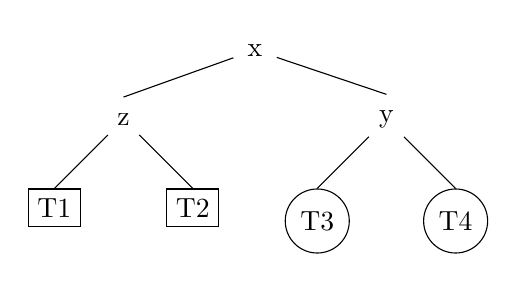
\begin{tikzpicture}[
				level distance = 2.5em,
				level 1/.style={sibling distance=9.5em},
				level 2/.style={sibling distance=5.0em},
				child anchor =north
				]
				\node[circle] (t1) {x}
				child { node[circle]   {z}
					child { node[draw=black, anchor = north]   {T1}
					}
					child { node[draw=black, anchor = north]   {T2}
					}
			}
				child { node[circle]   {y}
					child { node[circle, anchor = north, draw=black] {T3}}
					child { node[circle, anchor = north, draw=black] {T4}
					}
				};
			\end{tikzpicture}
		\column{0.455\textwidth}
		\begin{itemize}
			\item We can now rotate some stuff around :)
			\item Notice that the subtrees have not changed.
				\begin{itemize}
					\item $T1,T3,T4$ have a height of $h$
					\item $T2$ has a height of $h-1$
						\pause
					\item $z$ now has a height of $h+1$
					\item $y$ now has a height of $h+1$
					\item $x$ now has a height of $h+2$
				\end{itemize}
		\end{itemize}
			
	\end{columns}

	
\end{frame}

\begin{frame}
	\frametitle{Let's help ourselves}
	\begin{columns}
		\column{0.455\textwidth}
			
			\begin{tikzpicture}[
				level distance = 2.5em,
				level 1/.style={sibling distance=9em},
				level 2/.style={sibling distance=4.5em},
				level 3/.style={sibling distance=3em},
				level 4/.style={sibling distance=2em},
				]
				\node[circle] (t1) {12}
				child { node[circle]   {3}
					child { node[circle] {$\square$} }
					child { node[circle] {9}
						child { node[circle] {$\square$} }
						child { node[circle] {$\square$} }
					}
				}
				child { node[circle]   {25}
					child { node[circle] {14}
						child { node[circle] {$\square$} }
						child { node[circle] {$\square$} }
					}
					child { node[circle] {29}
						child { node[circle] {26}
							child { node[circle] {$\square$} }
							child { node[circle] {27}}
						}
						child { node[circle] {32}
							child { node[circle] {$\square$} }
							child { node[circle] {$\square$} }
						}
					}
				};
			\end{tikzpicture}
		\column{0.455\textwidth}
		\begin{itemize}
			\item Let's draw the non-existing leafs!
			\item This will help us identify what to rotate :)
				\pause
			\item And let's do this on the board.
		\end{itemize}
	\end{columns}
\end{frame}

\begin{frame}
	\frametitle{Phew...}
	\begin{center}
		
\includegraphics[width=0.5\textwidth]{images/relief.png}\\
		\hspace*{15pt}\hbox{\scriptsize Image By:\thinspace{\itshape Twitter}}
	\end{center}
	
\end{frame}

\begin{frame}
	\frametitle{Deletion}
	\framesubtitle{No! Not another}
		\begin{block}{Deleting a node}
			Also requires just one rotation to fix the imbalance.
		\end{block}	
		\pause
			\begin{block}{Tutorial time}
			  But we'll save that for the tutorial tomorrow.	
			\end{block}	
\end{frame}


\begin{frame}
	\frametitle{Binary Search Trees}
	\begin{center}
		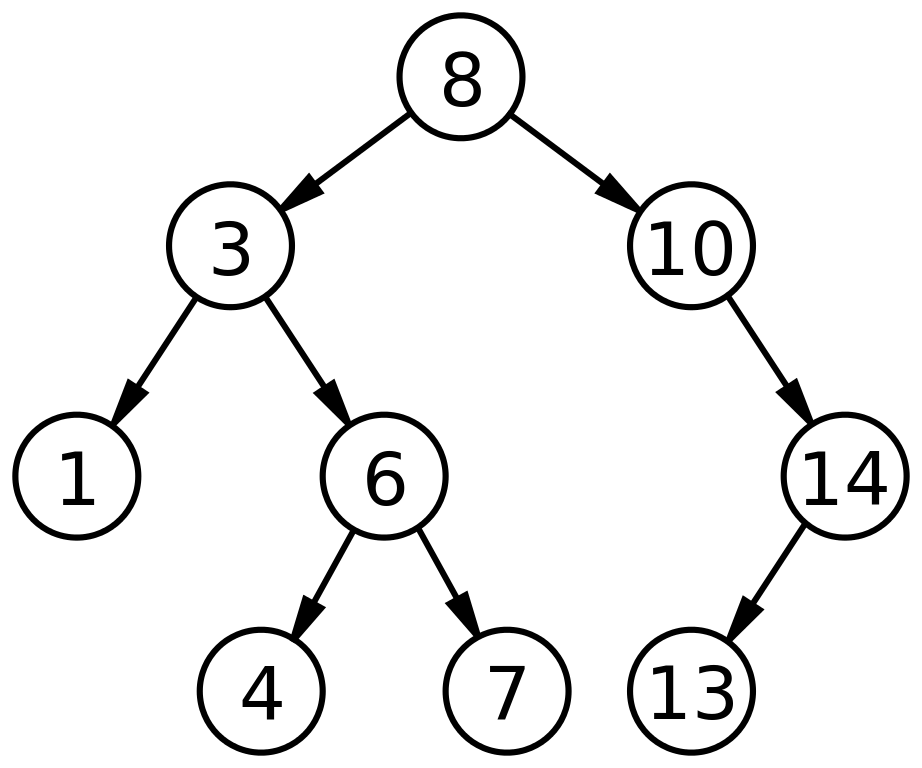
\includegraphics[width=0.5\textwidth]{images/btree.png}\\
		\hspace*{15pt}\hbox{\scriptsize Image By:\thinspace{\itshape Derrick Coetzee}}
		% https://en.wikipedia.org/wiki/File:Binary_search_tree.svg
	\end{center}
\end{frame}

\begin{frame}
	\frametitle{Binary Search Trees}
	
	\begin{block}{Binary \alert{Search} Trees}
		\begin{itemize}
			\item Every node has at most 2 children.
				\pause
			\item The left descendants have a smaller value than the node.
			\item The right descendants have a larger value than the node.
		\end{itemize}
	\end{block}	
	\pause
	\begin{columns}
		\column{0.455\textwidth}

		\begin{tikzpicture}[
			level distance = 2.5em,
			level 1/.style={sibling distance=9em},
			level 2/.style={sibling distance=4.5em},
			level 3/.style={sibling distance=2.25em},
			]
			\node[circle] (t1) {12}
			child { node[circle]   {3}
				child { node[circle] {2}}
				child { node[circle] {9}}
			}
			child { node[circle]   {25}
				child { node[circle] {14}}
				child { node[circle] {29}
					child { node[circle] {26}}
					child { node[circle] {32}}
				}
			};
		\end{tikzpicture}
		\column{0.455\textwidth}

		\begin{block}{Is it full?}
			Is this tree a binary search tree?
		\end{block}
		\pause
		\begin{block}{}
			Yes :)	
		\end{block}
	\end{columns}
\end{frame}

\begin{frame}
	\frametitle{Searching in a Binary SearchTree}
	
	\vspace{-20pt}
	\begin{overlayarea}{\textwidth}{\textheight}
		\begin{block}{Searching}
			So, how quickly can we search for an item in a Binary Search Tree?
			\only<1>{
			\begin{enumerate}[A.]
				\item $\Theta(\log h)$
				\item $\Theta(h)$
				\item $\Theta(\log n)$
				\item $\Theta(n)$
				\item $\Theta($\textit{I don't know man}$)$
			\end{enumerate}
		}
		\end{block}
		\pause
		\lstinputlisting{src/search_btree.py}
		\pause
	\vspace{-10pt}
		\begin{block}{Only one path}
			So $\Theta(h)$
		\end{block}
	\end{overlayarea}
\end{frame}

\begin{frame}
	\frametitle{MinMaxing}
	
	\begin{overlayarea}{\textwidth}{\textheight}
		\begin{block}{Minmaxing like a real gamer}
			So, how quickly can we find the minimum or maximum in a Binary Search Tree?
			\only<1>{
			\begin{enumerate}[A.]
				\item $\Theta(\log h)$
				\item $\Theta(h)$
				\item $\Theta(\log n)$
				\item $\Theta(n)$
				\item $\Theta($\textit{Something?}$)$
			\end{enumerate}
		}
		\end{block}
		\pause
		\lstinputlisting{src/minmax_btree.py}
		\pause
		\begin{block}{Only one path}
			So $\Theta(h)$
		\end{block}
	\end{overlayarea}
\end{frame}

\begin{frame}
	\frametitle{Inserting or Deleting an item}

	\begin{block}{Inserting an item}
		Find the right place in $\Theta(h)$ time, then put it there.
	\end{block}	

	\pause
	\begin{block}{Deleting an item}
		Find the item in $\Theta(h)$ time, then move either the left or right child up one level (and continue this down the
		path to a leaf).
	\end{block}	
	\pause
		\begin{block}{Sorting the list}
			Oh and by the way, this is where the in-order traversal can get us a sorted list of all items in the tree!
		\end{block}	
\end{frame}


\begin{frame}
	\frametitle{So in summary}
	\begin{tabular}{r | l}
		Operation & Time \\
		\midrule
		Insert & $\Theta(h)$ \\
		Delete & $\Theta(h)$ \\
		Search & $\Theta(h)$ \\
		Min & $\Theta(h)$ \\
		Max & $\Theta(h)$ \\
	\end{tabular}
	\pause	
	\begin{block}{So how bad is it?}
		What is the worst-case $h$, and how do we get that?
	\end{block}
	\pause
	\begin{block}{Inserting a sorted list}
		Insert a sorted list, and what happens? \\
		\pause 
		We get a tree with only right children (or only left if the list is sorted descendingly).
	\end{block}
	
\end{frame}


\begin{frame}
	\frametitle{Generalising a bit}
		\begin{block}{Multiway search tree}
			\begin{itemize}
				\item Each node of $T$ has \textit{at least} 2 children (except for leaves of course).
				\item Each $d$-node (where $d$ is the amount of children the node has), stores $d-1$ values in increasing value.
				\item Between two keys $i$ and $i+1$ stored in the node, is rooted a tree that contains only keys $k$ such that
					$k_i \leq k \leq k_{i+1}$.
			\end{itemize}
			
		\end{block}	

		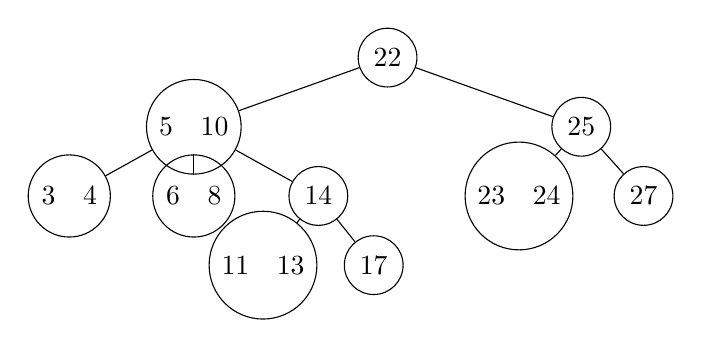
\begin{tikzpicture}[
			level distance = 2.5em,
			level 1/.style={sibling distance=14em},
			level 2/.style={sibling distance=4.5em},
			level 3/.style={sibling distance=2.25em},
			level 3/.style={sibling distance=4em},
			]
			\node[circle, draw] (t1) {22}
			child { node[circle, draw]   {5\quad10}
				child { node[circle, draw] {3\quad4}}
				child { node[circle, draw] {6\quad8}}
				child { node[circle, draw] {14}
					child { node[circle, draw] {11\quad13}}
					child { node[circle, draw] {17}}
				}
			}
			child { node[circle, draw]   {25}
				child { node[circle, draw] {23\quad24}}
				child { node[circle, draw] {27}}
			};
		\end{tikzpicture}
	
\end{frame}

\begin{frame}
	\frametitle{Practice?}
	
		\begin{block}{What should you know?}
			\begin{itemize}
				\item You should be able to search for items in a multiway search tree.
				\item And in the lab you will practice a bit with inserting nodes. Read the book carefully, it's not trivial!
				\item On the computer exam, we will not ask you to implement insertion or deletion in multiway search trees.
			\end{itemize}
		\end{block}	
\end{frame}


\begin{frame}
	\frametitle{Recap}
	
		\begin{block}{Binary Trees}
			\begin{itemize}
				\item Every node has at most 2 children.
					\pause
				\item One \textit{left} child and one \textit{right} child.
			\end{itemize}
		\pause
		A binary tree is \textit{proper} or \textit{full} if all nodes have either 0 or 2 children.
		\end{block}	
		\pause
		\begin{columns}
			\column{0.455\textwidth}
				
			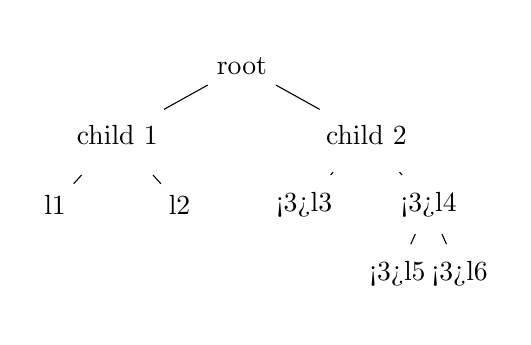
\begin{tikzpicture}[
				level distance = 2.5em,
				level 1/.style={sibling distance=9em},
				level 2/.style={sibling distance=4.5em},
				level 3/.style={sibling distance=2.25em},
			]
			\node[circle] (t1) {root}
				child { node[circle]   {child 1}
					child { node[circle] {l1}}
					child { node[circle] {l2}}
				}
				child { node[circle]   {child 2}
					child { node[circle] {\alert<3>{l3}}}
					child { node[circle] {\alert<3>{l4}}
						child { node[circle] {\alert<3>{l5}}}
						child { node[circle] {\alert<3>{l6}}}
					}
				};
			\end{tikzpicture}
			\column{0.455\textwidth}
				
			\begin{block}{Is it full?}
				Is this tree full?
			\end{block}
			\begin{block}{}
				Yes :)	
			\end{block}
		\end{columns}
\end{frame}

\begin{frame}
	\frametitle{Recap of Trees}
	\begin{columns}
		\column{0.405\textwidth}
			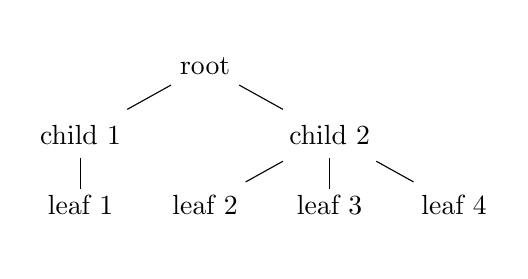
\begin{tikzpicture}[
				level distance = 2.5em,
				level 1/.style={sibling distance=9em},
				level 2/.style={sibling distance=4.5em},
				level 3/.style={sibling distance=2.25em},
			]
			\node[circle] (t1) {root}
				child { node[circle] {child 1}
					child { node[circle] {leaf 1}}
				}
				child { node[circle] {child 2}
					child { node[circle] {leaf 2}}
					child { node[circle] {leaf 3}}
					child { node[circle] {leaf 4}}
				};
			\end{tikzpicture}
		\column{0.555\textwidth}
		\begin{itemize}
			\item The \textit{root node} is the node that has no \textit{parent}.
			\item A node can have \textit{children}.
			\item A node without children is called a \textit{leaf}.
			\item Two nodes with the same \textit{parent} are \textit{siblings}.
			\item \textit{Descendants} are found by repeatedly following child-relations.
			\item \textit{Ancestors} are found by repeatedly following parent-relations.
		\end{itemize}
	\end{columns}
\end{frame}

%%%%%%%%%%%%%%%%%%%%%%%%%%%%%%%%%%%%%%%%%%%%%%%%%%%%%%%%%%%%%%%%%%%%%%
\begin{frame}[fragile]\frametitle{}
\begin{center}
{\Large Heaps}
\end{center}

\end{frame}


\begin{frame}
	\frametitle{Heaps}
	\framesubtitle{XKCD Tree: \url{https://xkcd.com/835}}
	\begin{center}
		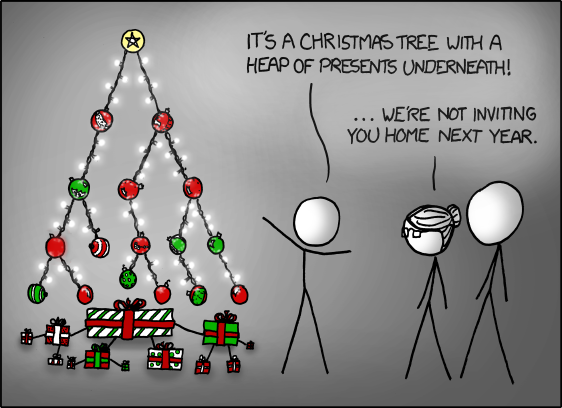
\includegraphics[width=0.6\textwidth]{images/tree.png}\\
	\end{center}
\end{frame}

\begin{frame}
	\frametitle{Heaps}
		\begin{block}{Heaps}
			We impose extra constraints and create a \textit{heap}:
			\begin{itemize}
				\item \textbf{Heap-order property:} For all nodes: The item stored in a node is greater than the item stored in its parent.
				\item \textbf{Complete Binary Tree property:} The tree is \textit{complete}: Meaning all layers are full, except possibly the last one which has only
					nodes in the left-most positions. 
			\end{itemize}
			\pause
			In this way, it is called a \textit{min-heap}. A \textit{max-heap} has the largest key in the root.
		\end{block}	
		\pause
		\begin{columns}
			\column{0.455\textwidth}

			\begin{tikzpicture}[
				level distance = 2.5em,
				level 1/.style={sibling distance=9em},
				level 2/.style={sibling distance=4.5em},
				level 3/.style={sibling distance=2.25em},
				]
				\node[circle] (t1) {1}
				child { node[circle]   {12}
					child { node[circle] {14}}
				}
				child { node[circle]   {4}
					child { node[circle] {5}}
					child { node[circle] {17}}
				};
			\end{tikzpicture}
			\column{0.455\textwidth}

			\begin{block}{Is it full?}
				Is this a correct min-heap?
			\end{block}
			\pause
			\vspace{-10pt}
			\begin{block}{Nope}
				No, as we do not use the left-most spots in the bottom layer.
			\end{block}
		\end{columns}
\end{frame}

\begin{frame}
	\frametitle{A use case}
	\framesubtitle{Me and my books, part 3}
	\begin{columns}
		\column{0.455\textwidth}
	\begin{center}
				\alt<5->{
					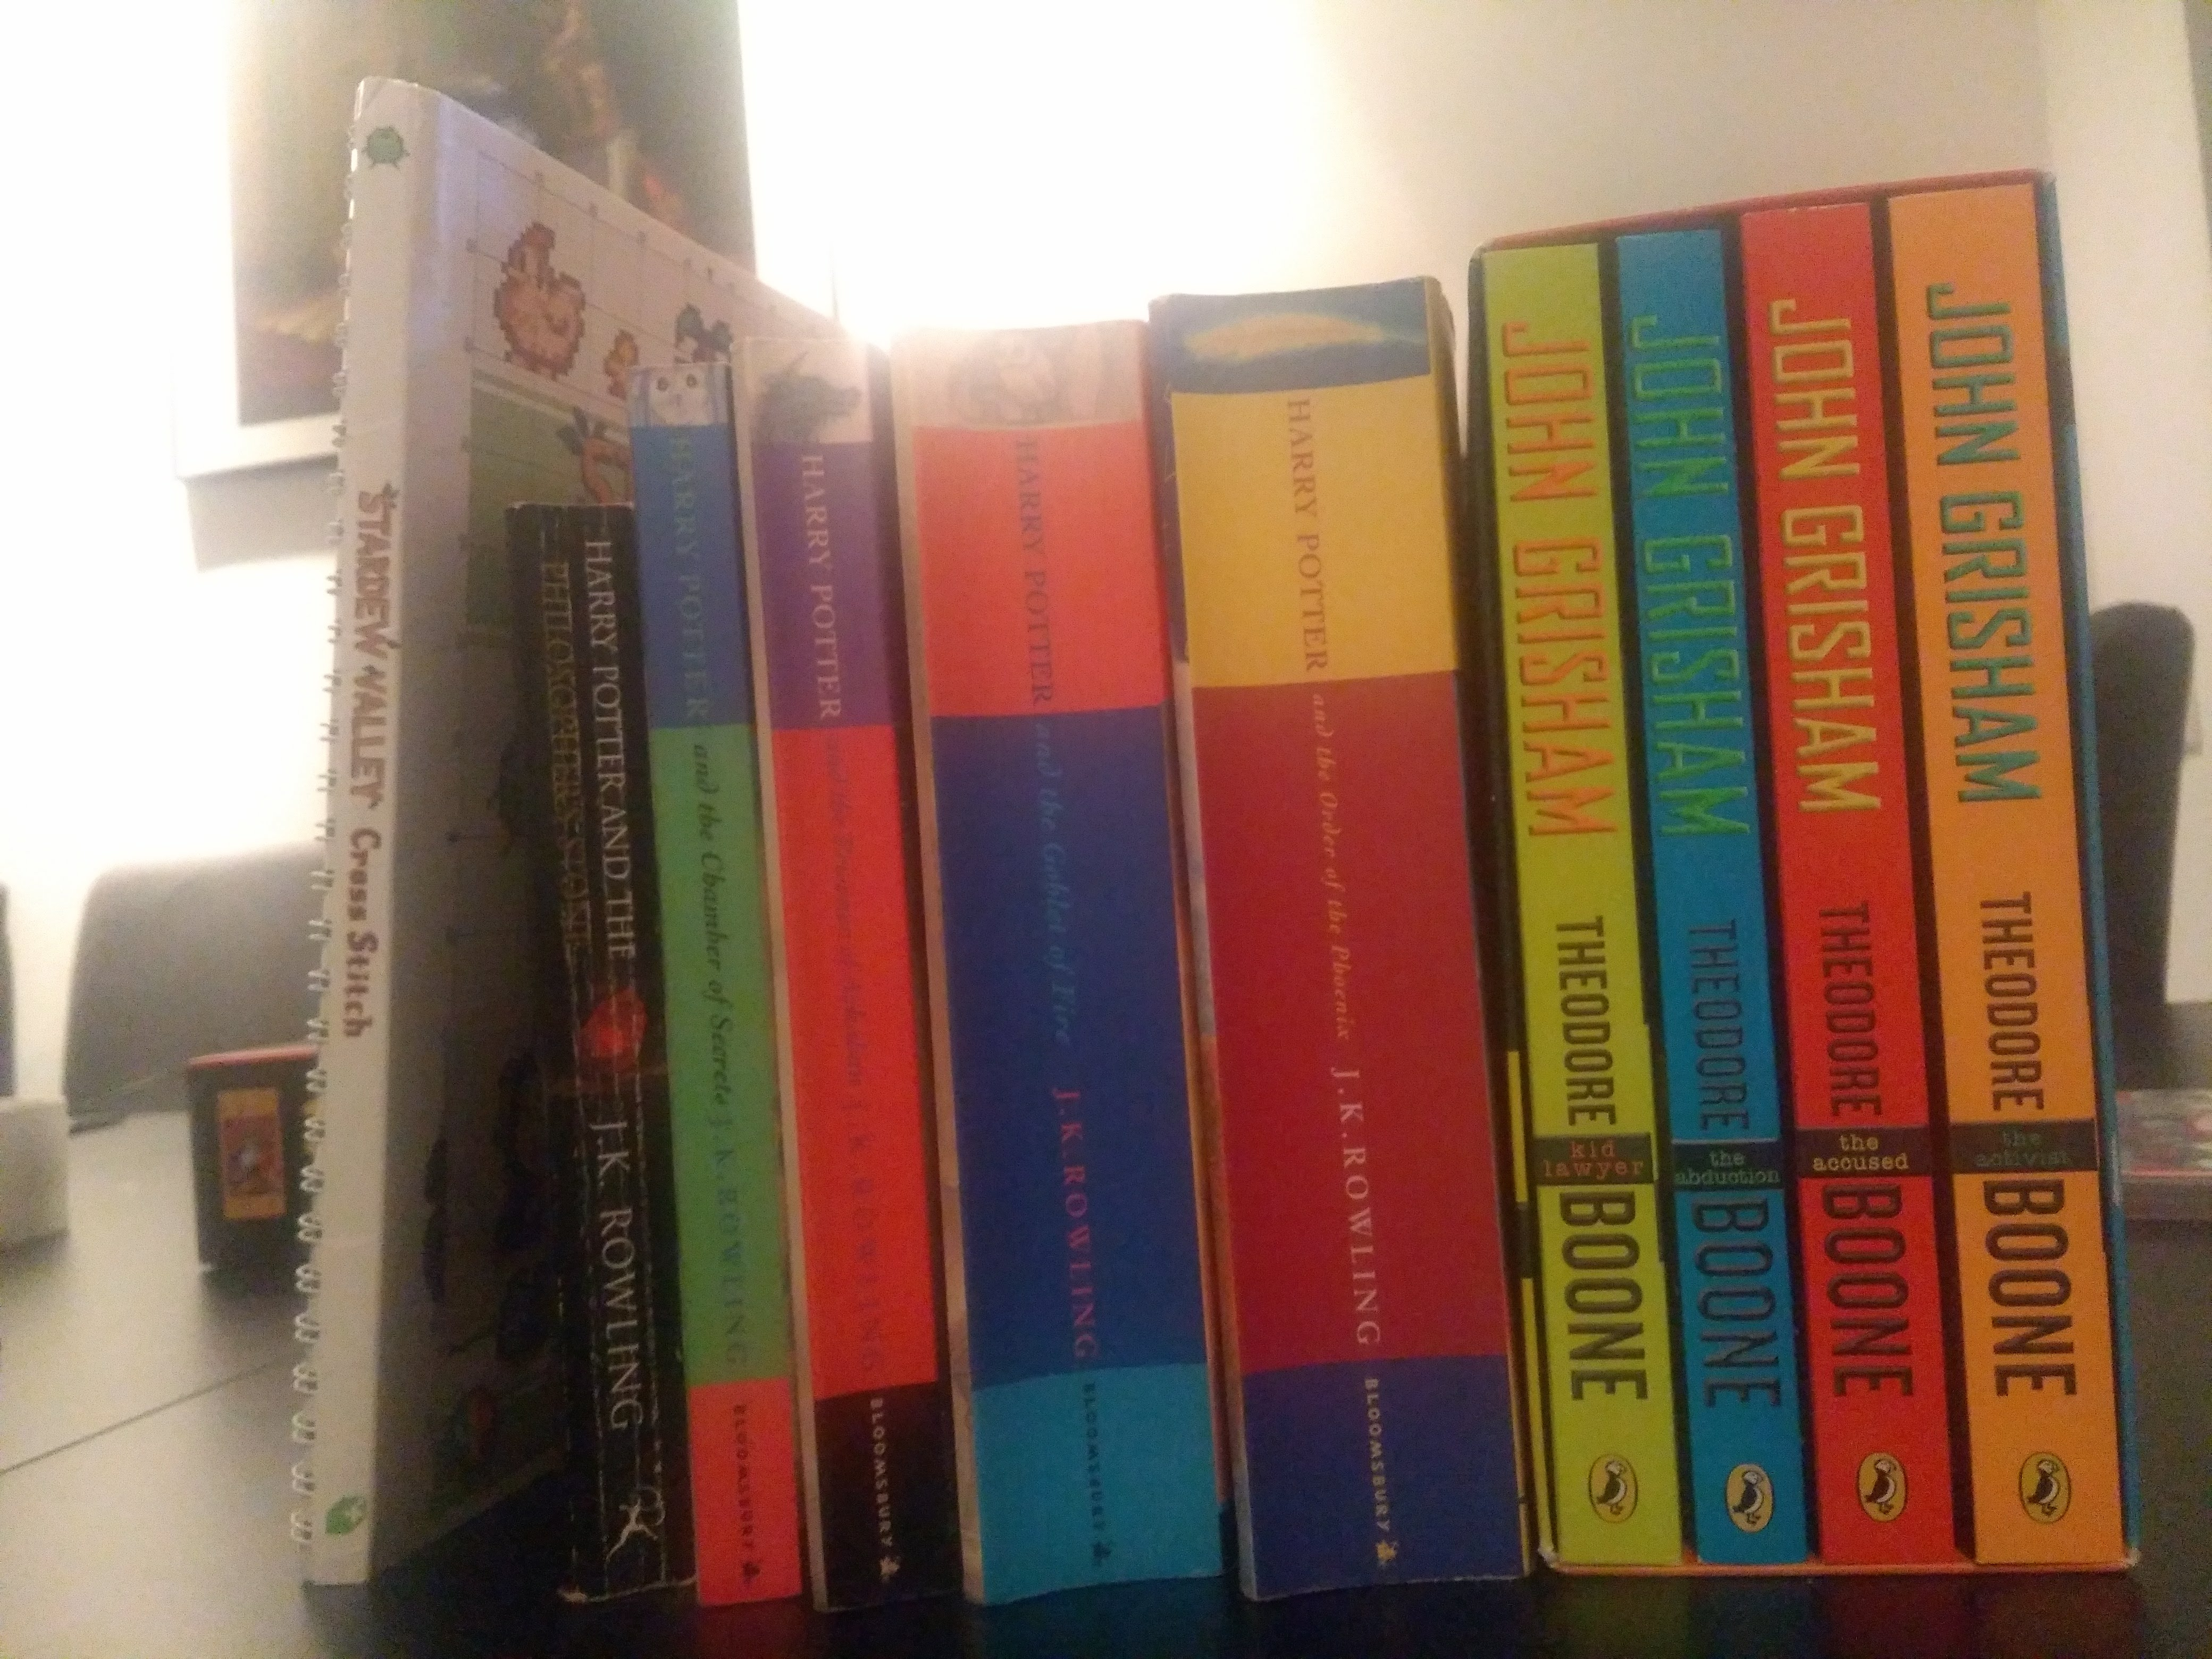
\includegraphics[width=\textwidth]{images/books_read.jpg}\\
					}{
					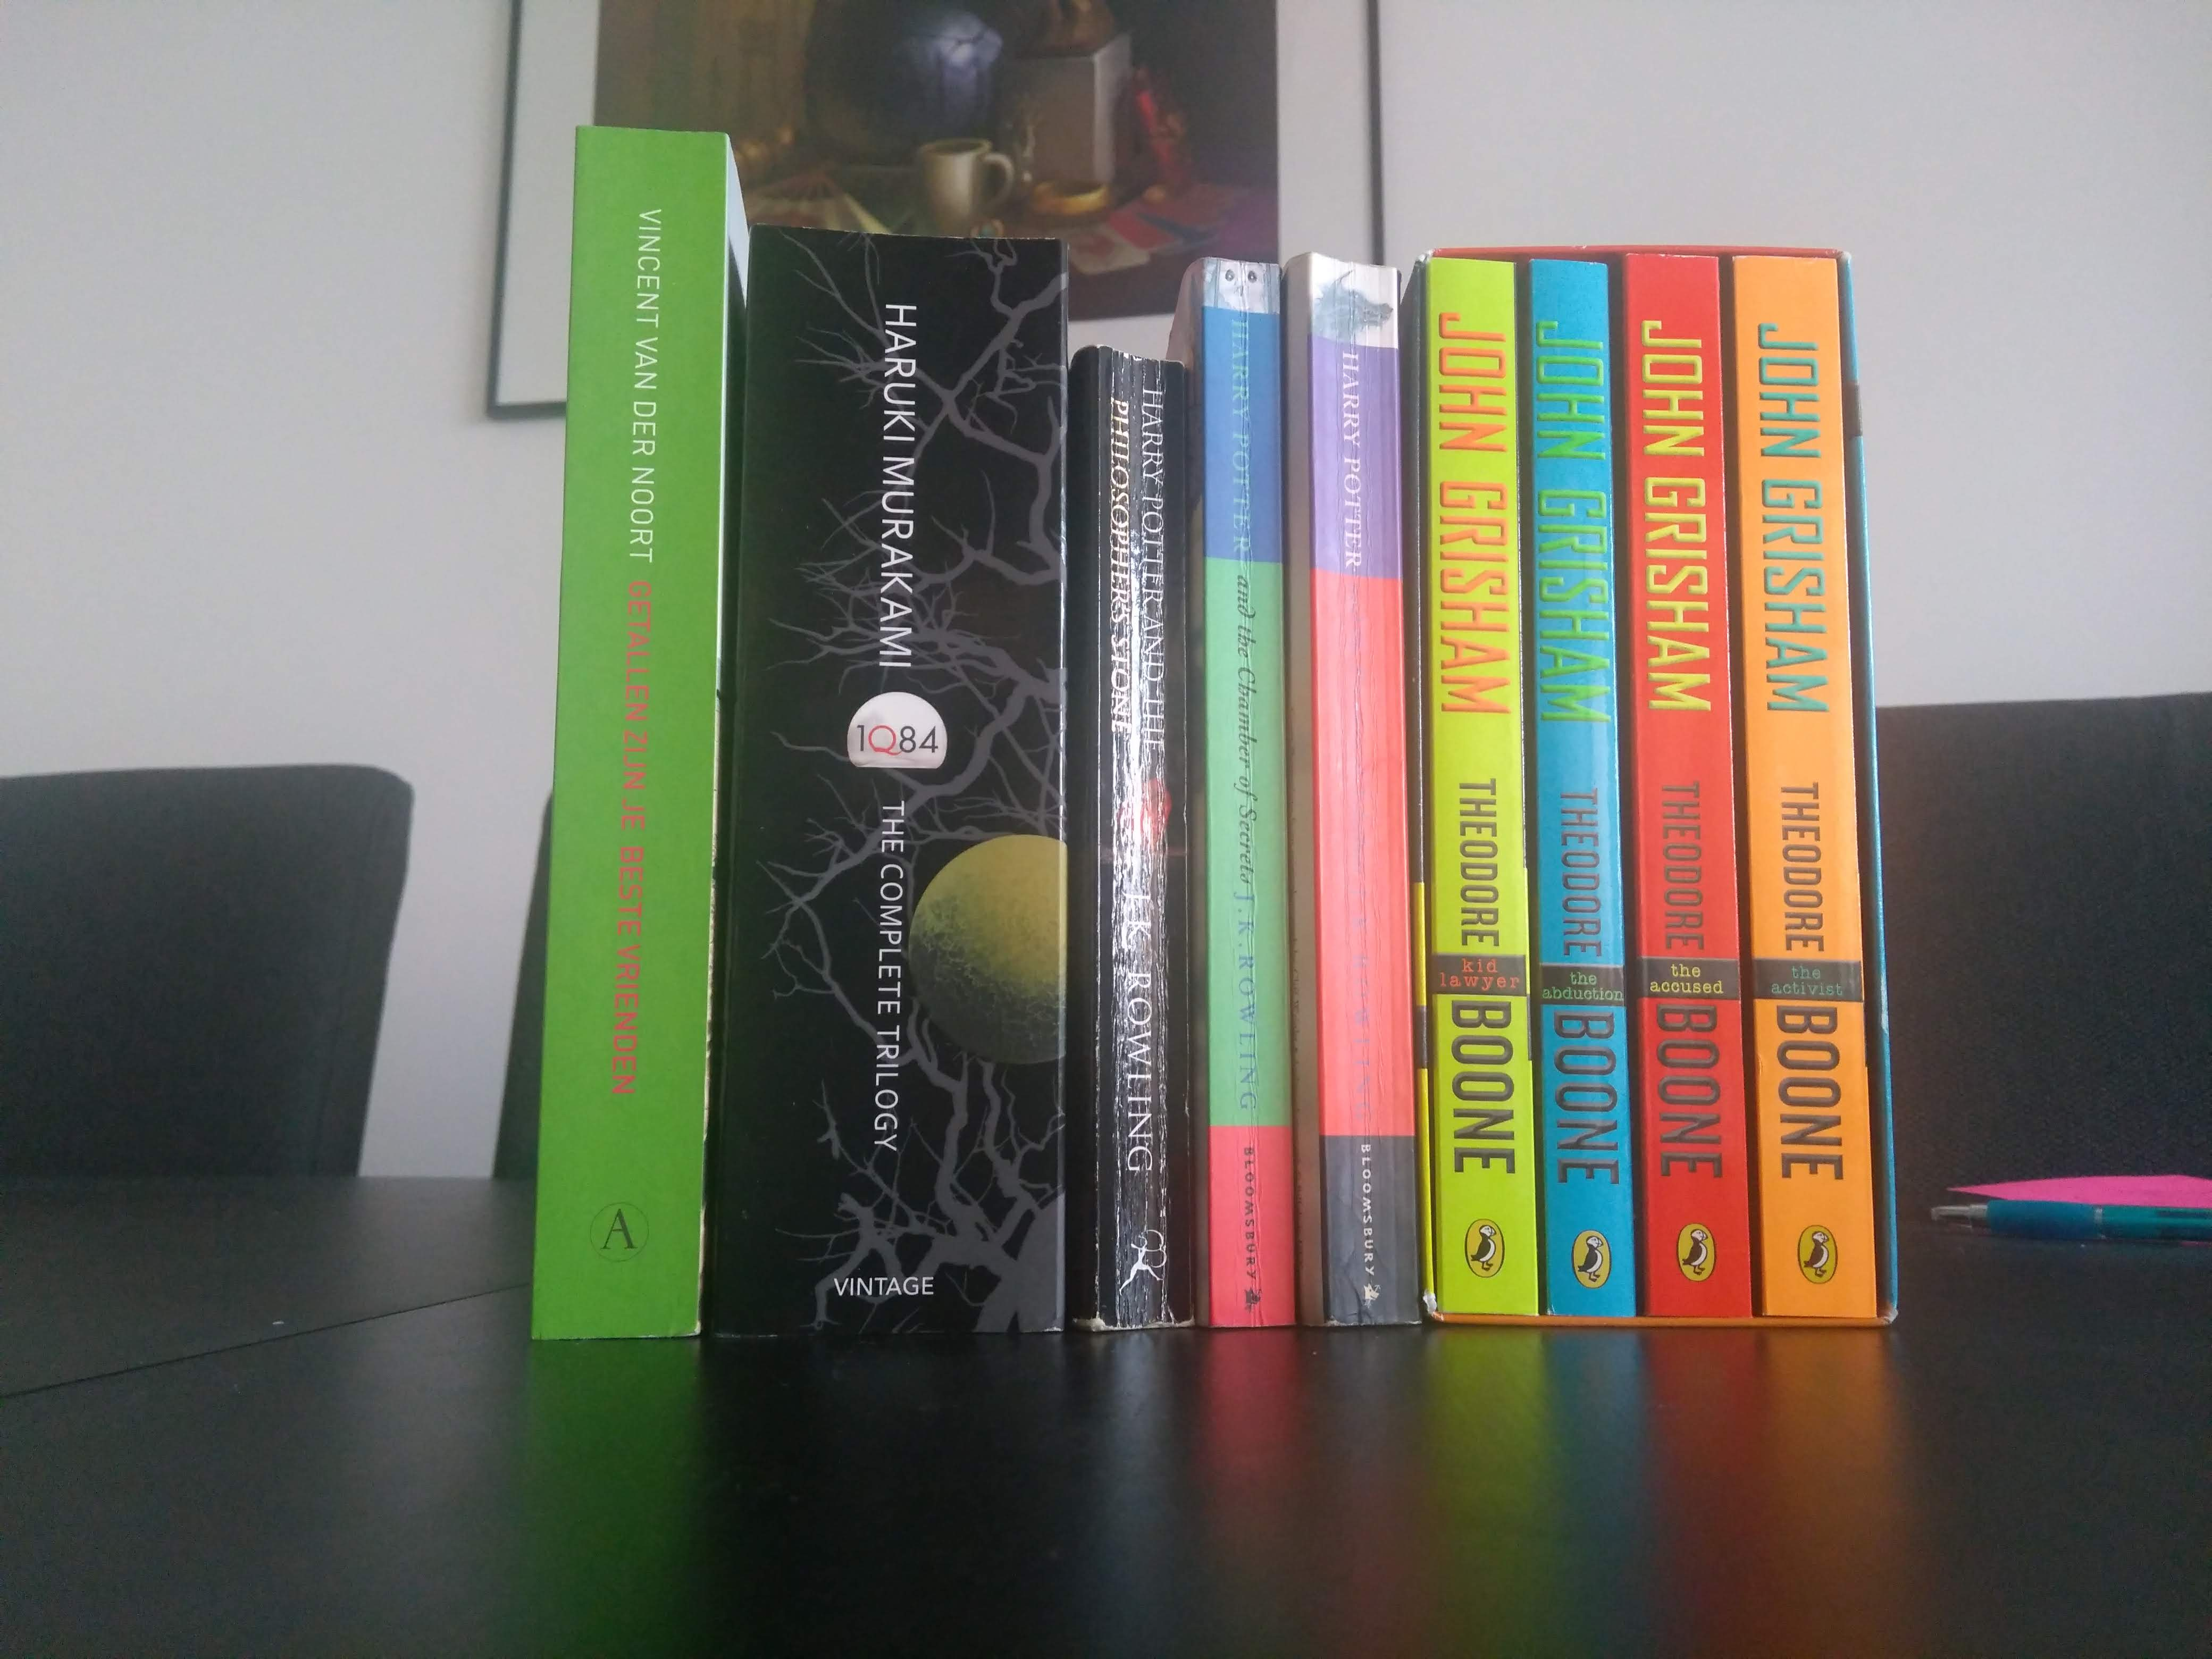
\includegraphics[width=\textwidth]{images/books_unread.jpg}\\
					}
		\hspace*{15pt}\hbox{\scriptsize Image By:\thinspace{\itshape Stefan Hugtenburg}}
		\hspace*{15pt}\hbox{\scriptsize Bookcovers and picture in the back by others}
	\end{center}
		\column{0.455\textwidth}
		\begin{itemize}
			\item There is more room for improvement.
				\pause
			\item A nice \alert{queue} of books.
				\pause
			\item After finishing one, I would take the next one from the left.
				\pause
			\item But what if a book should get \textit{priority}?
				\pause
			\item This uses a \textit{Priority Queue}, which we discuss in detail today.
		\end{itemize}
	\end{columns}
\end{frame}




\begin{frame}
	\frametitle{Bubbles!}
	\begin{center}
		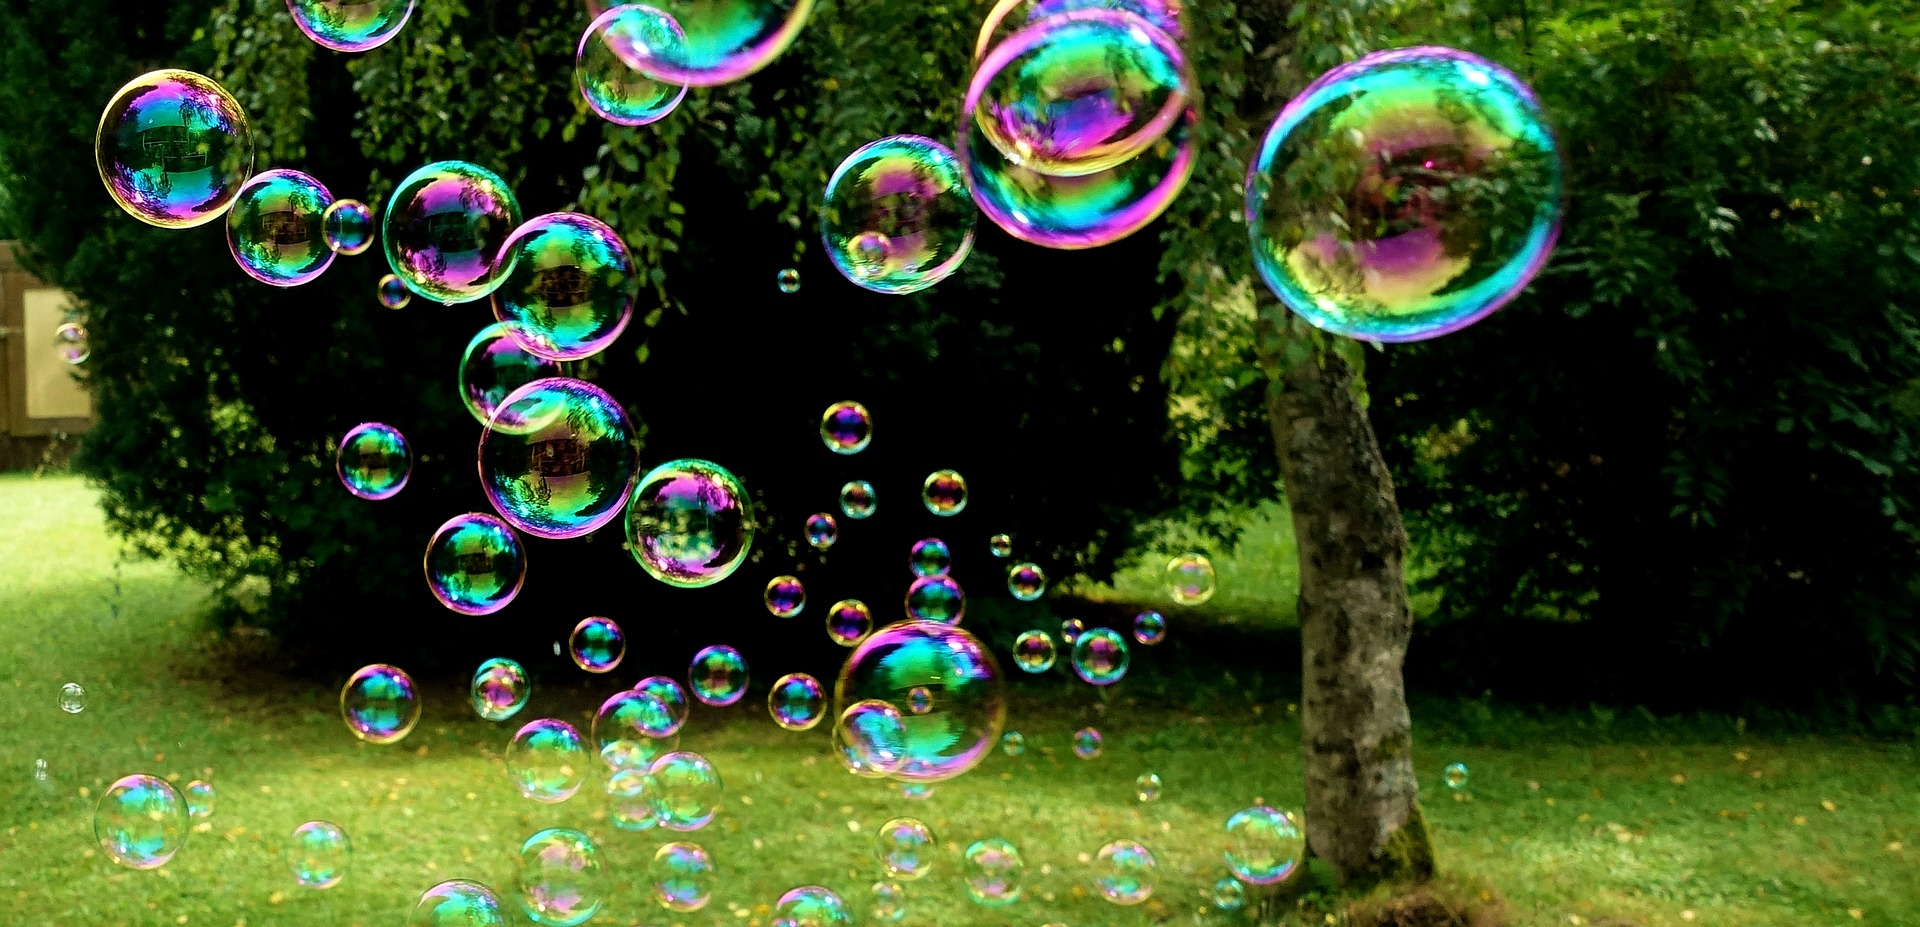
\includegraphics[width=0.8\textwidth]{images/bubble.jpg}\\
		\hspace*{15pt}\hbox{\scriptsize Image By:\thinspace{\itshape Alexas Fotos}}
		% https://pixabay.com/photos/soap-bubbles-colorful-flying-3517247/
	\end{center}
\end{frame}

\begin{frame}
	\frametitle{\alt<2->{A PriorityQueue ADT}{A Heap ADT}}
		\begin{block}{Heap, Heap, Array}
			There is no heap ADT per sé, it's just a special type of tree.
		\end{block}	
		\pause
		\begin{block}{PriorityQueue}
			But there is one for a PriorityQueue (which we could implement using a heap):
			\begin{itemize}
				\item \texttt{size()} (or \texttt{len} in Python) to get the number of elements.
					\pause
				\item \texttt{add(item)} to insert an item into the queue.
					\pause
				\item \texttt{remove\_min()} to remove the smallest element from the queue.
					\pause
				\item \texttt{min()} to get the smallest element from the queue.
			\end{itemize}
		\end{block}	
\end{frame}

\begin{frame}
	\frametitle{An array-based Priority Queue}

	\vspace{-20pt}
	\begin{columns}[t]
		\column{0.455\textwidth}
		\lstinputlisting{src/pq_array.py}
		\column{0.455\textwidth}
		\pause
		\begin{block}{Array-based PQ}
			We can easily create a PQ based on an array (or list).
		\end{block}	
		\pause
			\begin{block}{No, bad line graph!}
				But this makes \texttt{min} and \texttt{remove\_min} linear time operations!
			\end{block}	
			\pause
			\begin{block}{Can we do better?}
				Can we do better by using a sorted array?
			\end{block}
	\end{columns}
\end{frame}

\begin{frame}
	\frametitle{An sorted array-based Priority Queue}

	\vspace{-20pt}
	\begin{columns}[t]
		\column{0.455\textwidth}
		\lstinputlisting{src/pq_sortedarray.py}
		\column{0.455\textwidth}
		\pause
		\begin{block}{Array-based PQ}
			We can easily create a PQ based on a sorted array (or list).
		\end{block}	
		\pause
			\begin{block}{No, bad line graph!}
				But this makes \texttt{remove\_min} and \texttt{add} linear time operations!
			\end{block}	
			\pause
			\begin{block}{Can we do better?}
				Can we do better by using a heap?
			\end{block}
	\end{columns}
\end{frame}

\begin{frame}
	\frametitle{Min in a heap}
	\begin{block}{Consider a heap}
		How do I implement \texttt{min} for my heap-based PQ?
		\begin{enumerate}[A.]
			\item Return the value in the root.
			\item Return the value of the left-most descendant.
			\item Return the value of the right-most descendant.
			\item Go over all elements and return the minimum.
		\end{enumerate}
	\end{block}
	
	
\end{frame}

\begin{frame}
	\frametitle{Adding in a heap}
	\begin{block}{Consider a heap}
		Consider the following heap:\\
		\begin{columns}
			\column{0.455\textwidth}
			\begin{tikzpicture}[
				level distance = 2.5em,
				level 1/.style={sibling distance=9em},
				level 2/.style={sibling distance=4.5em},
				level 3/.style={sibling distance=2.25em},
				]
				\node[circle] (t1) {1}
				child { node[circle]   {12}
					child { node[circle] {14}}
					child { node[circle] {17}}
				}
				child { node[circle]   {4}
					child { node[circle] {5}}
				};
			\end{tikzpicture}
			\column{0.455\textwidth}
			\pause
			If I insert the element $7$ here, what should I do?
		\end{columns}
	\end{block}
	\begin{block}{Just add it at the bottom-right!}
			\begin{tikzpicture}[
				level distance = 2.5em,
				level 1/.style={sibling distance=9em},
				level 2/.style={sibling distance=4.5em},
				level 3/.style={sibling distance=2.25em},
				scale=0.8, transform shape
				]
				\node[circle] (t1) {1}
				child { node[circle]   {12}
					child { node[circle] {14}}
					child { node[circle] {17}}
				}
				child { node[circle]   {4}
					child { node[circle] {5}}
					child { node[circle] {7}}
				};
			\end{tikzpicture}
	\end{block}
\end{frame}

\begin{frame}
	\frametitle{Adding in a heap}
	\begin{block}{Consider a heap}
		Consider the following heap:\\
		\begin{columns}
			\column{0.455\textwidth}
			\begin{tikzpicture}[
				level distance = 2.5em,
				level 1/.style={sibling distance=9em},
				level 2/.style={sibling distance=4.5em},
				level 3/.style={sibling distance=2.25em},
				]
				\node[circle] (t1) {1}
				child { node[circle]   {12}
					child { node[circle] {14}}
					child { node[circle] {17}}
				}
				child { node[circle]   {4}
					child { node[circle] {5}}
				};
			\end{tikzpicture}
			\column{0.455\textwidth}
			\pause
			If I insert the element $0$ here, what should I do?
		\end{columns}
	\end{block}
	\begin{block}{Just add it at the bottom-right!}
		\begin{columns}
			\column{0.455\textwidth}
			\begin{tikzpicture}[
				level distance = 2.5em,
				level 1/.style={sibling distance=9em},
				level 2/.style={sibling distance=4.5em},
				level 3/.style={sibling distance=2.25em},
				scale=0.8, transform shape
				]
				\node[circle] (t1) {1}
				child { node[circle]   {12}
					child { node[circle] {14}}
					child { node[circle] {17}}
				}
				child { node[circle]   {4}
					child { node[circle] {5}}
					child { node[circle] {0}}
				};
			\end{tikzpicture}
			\column{0.455\textwidth}
			\pause
			And now fix the damage we have caused :)
		\end{columns}
	\end{block}
\end{frame}

\begin{frame}
	\frametitle{Up-bubbling}

	\begin{block}{Fixing the damage}
		How can we fix the damage caused to the heap \textit{efficiently}?
		\begin{columns}
			\column{0.455\textwidth}
			\begin{tikzpicture}[
				level distance = 2.5em,
				level 1/.style={sibling distance=9em},
				level 2/.style={sibling distance=4.5em},
				level 3/.style={sibling distance=2.25em},
				scale=0.8, transform shape
				]
				\node[circle] (t1) {1}
				child { node[circle]   {12}
					child { node[circle] {14}}
					child { node[circle] {17}}
				}
				child { node[circle]   {4}
					child { node[circle] {5}}
					child { node[circle] {0}}
				};
			\end{tikzpicture}
			\column{0.455\textwidth}
			\pause
			\begin{enumerate}[A.]
				\item Swap it with the root element and then swap it down as needed.
				\item Repeatedly compare the new node with the siblings and swap if needed.
				\item Repeatedly compare the new node with the parent and swap if needed.
				\item We cannot, we have to rebuild the entire heap.
			\end{enumerate}
		\end{columns}
	\end{block}
\end{frame}

\begin{frame}
	\frametitle{Up-bubbling}

	\begin{block}{Fixing the damage}
		Repeatedly switch with the parent if needed.\\
		\begin{columns}
			\column{0.455\textwidth}
				
			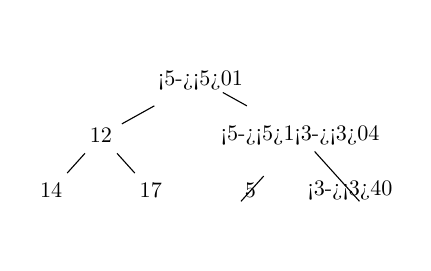
\begin{tikzpicture}[
				level distance = 2.5em,
				level 1/.style={sibling distance=9em},
				level 2/.style={sibling distance=4.5em},
				level 3/.style={sibling distance=2.25em},
				scale=0.8, transform shape
				]
				\node[circle] (t1) {\alt<5->{\alert<5>{0}}{1}}
				child { node[circle]   {12}
					child { node[circle] {14}}
					child { node[circle] {17}}
				}
				child { node[circle] {\alt<5->{\alert<5>{1}}{\alt<3->{\alert<3>{0}}{4}}}
					child { node[circle] {5}}
					child { node[circle] {\alt<3->{\alert<3>{4}}{0}}}
				};
			\end{tikzpicture}
			\column{0.455\textwidth}
			\only<6->{
			\begin{itemize}
				\item Notice how the left half of the tree has not been touched at all!
				\item Only one path changes!
			\end{itemize}	
	}
		\end{columns}
	\end{block}
\end{frame}

\begin{frame}
	\frametitle{Up-bubbling pt2}
			\begin{tikzpicture}[
				level distance = 2.5em,
				level 1/.style={sibling distance=9em},
				level 2/.style={sibling distance=4.5em},
				level 3/.style={sibling distance=2.25em},
				scale=0.8, transform shape
				]
				\node[circle] (t1) {6}
				child { node[circle]   {14}
					child { node[circle] {17}}
					child { node[circle] {21}}
				}
				child { node[circle]   {8}
					child { node[circle] {18}}
					child { node[circle] {9}}
				};
			\end{tikzpicture}
			\begin{block}{Where does it go?}
				Try to insert the element $10$ in this heap. Where does it end up?
				\begin{enumerate}[A.]
					\item As the root
					\item At depth 1
					\item At depth 2
					\item At depth 3
				\end{enumerate}
			\end{block}
\end{frame}

\begin{frame}
	\frametitle{Removing from a heap}
	\begin{block}{Consider a heap}
		Consider the following heap:\\
		\begin{columns}
			\column{0.455\textwidth}
			\begin{tikzpicture}[
				level distance = 2.5em,
				level 1/.style={sibling distance=9em},
				level 2/.style={sibling distance=4.5em},
				level 3/.style={sibling distance=2.25em},
				]
				\node[circle] (t1) {1}
				child { node[circle]   {12}
					child { node[circle] {14}}
					child { node[circle] {17}}
				}
				child { node[circle]   {4}
					child { node[circle] {5}}
					child { node[circle] {7}}
				};
			\end{tikzpicture}
			\column{0.455\textwidth}
			\pause
			If I want to remove the minimum, what should I do?
		\end{columns}
	\end{block}
	\begin{block}{Just remove it at the top!}
		\begin{columns}
			\column{0.455\textwidth}
			\begin{tikzpicture}[
				level distance = 2.5em,
				level 1/.style={sibling distance=9em},
				level 2/.style={sibling distance=4.5em},
				level 3/.style={sibling distance=2.25em},
				scale=0.8, transform shape
				]
				\node[circle] (t1) {$\square$}
				child { node[circle]   {12}
					child { node[circle] {14}}
					child { node[circle] {17}}
				}
				child { node[circle]   {4}
					child { node[circle] {5}}
					child { node[circle] {7}}
				};
			\end{tikzpicture}
			\column{0.455\textwidth}
			\pause
			And now fix the damage we have caused :)
		\end{columns}
	\end{block}
\end{frame}

\begin{frame}
	\frametitle{Fixing the damage}
	\begin{block}{Just remove it at the top!}
		\begin{columns}
			\column{0.455\textwidth}
			\begin{tikzpicture}[
				level distance = 2.5em,
				level 1/.style={sibling distance=9em},
				level 2/.style={sibling distance=4.5em},
				level 3/.style={sibling distance=2.25em},
				scale=0.8, transform shape
				]
				\node[circle] (t1) {$\square$}
				child { node[circle]   {12}
					child { node[circle] {14}}
					child { node[circle] {17}}
				}
				child { node[circle]   {4}
					child { node[circle] {5}}
					child { node[circle] {7}}
				};
			\end{tikzpicture}
			\column{0.455\textwidth}
			\pause
			What should we do?
			\begin{enumerate}[A.]
				\item Repeatedly move the smallest child up.
				\item First move the bottom right to the root and then repeatedly swap down with the smallest child.
				\item Always get the smallest element from the next layer and move it up (so not restricted to your children).
				\item Nothing, we should just rebuild the heap from scratch.
			\end{enumerate}
		\end{columns}
	\end{block}
	
\end{frame}

\begin{frame}
	\frametitle{Down-bubbling}

	\begin{block}{Fixing the damage}
		First move the bottom-right element to the top, then repeatedly bubble down.
		\begin{columns}
			\column{0.455\textwidth}
				
			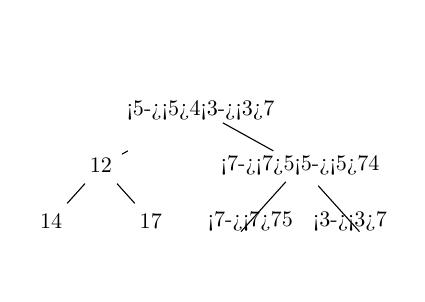
\begin{tikzpicture}[
				level distance = 2.5em,
				level 1/.style={sibling distance=9em},
				level 2/.style={sibling distance=4.5em},
				level 3/.style={sibling distance=2.25em},
				scale=0.8, transform shape
				]
				\node[circle] (t1) {\alt<5->{\alert<5>{4}}{{\alt<3->{\alert<3>{7}}{$\square$}}}}
				child { node[circle]   {12}
					child { node[circle] {14}}
					child { node[circle] {17}}
				}
				child { node[circle] {\alt<7->{\alert<7>{5}}{\alt<5->{\alert<5>{7}}{4}}}
					child { node[circle] {\alt<7->{\alert<7>{7}}{5}}}
					child { node[circle] {\alt<3->{\alert<3>{$\square$}}{7}}}
				};
			\end{tikzpicture}
			\column{0.455\textwidth}
			\only<8->{
			\begin{itemize}
				\item Notice how the left half of the tree has not been touched at all!
				\item Only one path changes, after the initial switch!
			\end{itemize}	
	}
		\end{columns}
	\end{block}
\end{frame}

\begin{frame}
	\frametitle{Down-bubbling pt2}
			\begin{tikzpicture}[
				level distance = 2.5em,
				level 1/.style={sibling distance=9em},
				level 2/.style={sibling distance=4.5em},
				level 3/.style={sibling distance=2.25em},
				scale=0.8, transform shape
				]
				\node[circle] (t1) {6}
				child { node[circle]   {14}
					child { node[circle] {17}
						child { node[circle] {19}}
					}
					child { node[circle] {21}
					}
				}
				child { node[circle]   {8}
					child { node[circle] {18}}
					child { node[circle] {12}
					}
				};
			\end{tikzpicture}
			\begin{block}{Where does it go?}
				Remove the minimum from the heap, where does $18$ end up?
				\begin{enumerate}[A.]
					\item As the root
					\item At depth 1
					\item At depth 2
					\item At depth 3
				\end{enumerate}
			\end{block}
\end{frame}
